\documentclass[11pt]{article}
\usepackage{epsfig}
\usepackage{graphicx}
\usepackage{rotating}
\usepackage{amsmath,amsthm}
\usepackage{array}
\usepackage{multirow}
\usepackage{url}
\usepackage{appendix}
\usepackage{algorithm}
\usepackage{algorithmic}
\usepackage{placeins} % FloatBarrier
\usepackage{comment}
\usepackage{enumerate} % Fancy enumeration
\usepackage{appendix}
\usepackage{listings}


\newcommand{\vs}{\vspace{0.1in}}


\usepackage{float}
%\floatstyle{boxed}
%\restylefloat{figure}
%\usepackage{morefloats}

\usepackage{caption}


\lstset{breaklines=true}


\oddsidemargin=0in
\evensidemargin=0in
\textwidth=6.5in
%\textwidth=6.42in (if no footnote)
\textheight=8.75in
%\textheight=9.1in (if no footnote)
\topmargin=-0.5cm
%\topmargin=0.5in
\footskip=1.0cm
\headheight=0pt
%\newcommand{\comment}[1]{}

\setlength{\extrarowheight}{5pt}

\theoremstyle{definition}
\newtheorem{definition}{Definition}
\newtheorem*{examples}{Examples}
\newtheorem{example}{}

\begin{document}

\title{An Empirical Evaluation of Denoising\\Techniques for Streaming Data}

\date{\today}

%

\author{Jeremy Luke Thompson\thanks{United States Air Force Academy and Lawrence Livermore National Laboratory}}


%\vfill
%\vspace{2.0in}
\maketitle


\begin{abstract}
  We investigate denoising techniques for streaming data. This is
  data that is analyzed while it is collected. We consider
  spatial filters, such as the box filter, Gaussian smoothing, and the
  bilateral filter; frequency-based techniques, such as fast Fourier
  transform and wavelet transform, combined with thresholding of the
  coefficients; and a statistical neighborhood filter, the non-local
  means algorithm. We discuss practical concerns for incremental
  implementation, such as edge treatment, incremental
  updating, and parameter stability. These methods are
  applied to both synthetic data and real world data. Based on several
  carefully designed experiments, we note situations when these
  methods could fail and make recommendations for their use with real
  world data. Specifically, we suggest the use of the bilateral filter
  alone or a combination of the bilateral filter and non-local means algorithm.
\end{abstract}

%\thispagestyle{empty} %\vspace{2.0in}

%\vfill \eject

\clearpage

%\thispagestyle{empty}

\tableofcontents
\thispagestyle{empty}

\clearpage

\pagestyle{plain}
\pagenumbering{arabic}


%%%%%%%%%%%%%%%%%%%%%%%%%%%%%%%%%%%%%%%%%%%%%%%%%%%%%%%%%%%%%%%%%%%%%%%%%%


 
\section{Introduction}


A time series is any temporally ordered series of observations.
Frequently, as when collecting observations of various real world
phenomenon, these observations will be contaminated with a variety of
errors, or noise, such as sampling and processing errors. In
traditional time series data, the denoising is done after the data has
been collected. As a result, there is an opportunity to try different
denoising techniques and experiment with different parameters to
select a method that works best for a data set. Our focus in this report is
on streaming data, where the data is analyzed as it is collected. We therefore consider techniques that can be applied
incrementally.  We discuss multiple classes of techniques and
practical considerations for incremental implementation such as edge
treatment and incremental updating. We investigate how we can select
the parameters for the algorithms so that the same parameters can be
used over time, while yielding acceptable results.  Additionally, we
assess the performance of these techniques in the context of peak
signal to noise ratio for known time series with added noise and
optimal parameter stability.


Many deniosing techniques rely upon an estimate of the variance of the
distribution this random noise comes from, typically assumed to be
Gaussian. Gasser, et al.~\cite{Gasser86} describe a method for
estimating this unknown value based upon the sum of squared
differences between the observed data and linear interpolations
approximating the true values of the time series. In this report, we
use the notation $y_i$ for the values of the time series at time index
$i$. For a time series with $N$ values, starting at $i = 0$, the
estimated noise variance as given in ~\cite{Gasser86} is:


\begin{displaymath}
  \hat{\sigma} ^2_n = \frac{2}{3 \left( N - 2 \right)} \sum _{i = 1} ^{N - 2} \left( \frac{1}{2} y_{i - 1} - y_i + \frac{1}{2} y_{i + 1} \right) ^2
\label{eqn:noise_var}
\end{displaymath}

As discussed later in the report, we use this estimate to set the
parameters of some of the denoising techniques we investigate.  There
are, naturally, a variety of other techniques~\cite{Donoho94,immerkaer96:noise} for
noise variance estimation, with different levels of robustness and
computational difficultly. We use Equation~\ref{eqn:noise_var} because
of its simplicity.

The report is organized as follows. A description of the denoising
techniques we will use is given in Section \ref{denoise}. We discuss
the design of experiment for empirical comparison of these denoising
methods in Section \ref{design}. Experimental results on both
synthetic and real world data are discussed in Section \ref{results} and \ref{results2}.
We conclude our evaluation and provide recommendations along with
suggestions for future work in Section \ref{conclusion}.

%=============================================
\section{Denoising techniques}\label{denoise}
%=============================================

There are a variety of denosing techniques, and they fit into three
broad categories: local smoothing filters, frequency coefficient
thresholding techniques, and statistical neighborhood filters. We
discuss three spatial filters: the box filter, Gaussian filter, and
bilateral filter; two frequency techniques: Fourier transform and
wavelet transform, with coefficient thresholding; and one statistical
neighborhood filter, the non-local means algorithm. Besides these common methods, we
propose combination approaches derived from them.

The color convention for charts in this report is black for the true
time series values, if known, blue for the noisy time series values,
red for the denoised time series values, and cyan for the residuals,
the difference between the noisy and denoised time series values.  

%============================
\subsection{Spatial filters}
%============================
%-------------------------
\subsubsection{Box filter} 
%-------------------------
The box filter is the simplest denoising technique and is a uniformly
weighted moving average of the time series. This technique works best
in time series with true values that do not change rapidly so the
noise averages to zero over an interval while the true time series
values remain relatively unchanged. Smoothed values are given by

\begin{displaymath}
s_i = \sum _{j \in I} w \left(i, j \right) y_j,
\end{displaymath}

\noindent
where the weights are given by the function

\begin{displaymath}
w\left(i, j\right) = \frac{1}{\lvert I \rvert},
\end{displaymath}

\noindent
and $\lvert I \rvert$ is the size of the time interval, or window, of
the filter. Typically the interval is symmetric about the point of
interest, which means $\lvert I \rvert$ is odd. In this technique, the
interval size is a parameter to be chosen by the analyst. Figure
\ref{boxdemo} shows the weighting scheme for the box filter.


\begin{figure}[h!]
\centering
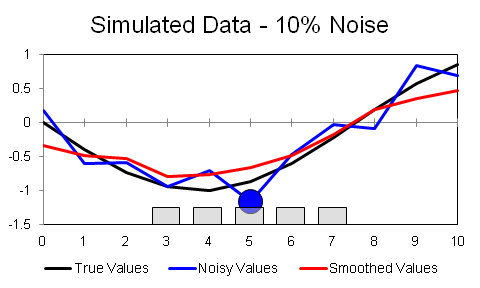
\includegraphics[width = 0.4 \textwidth]{BoxDemo.png}
\caption{Box Filter Weighting Scheme}
\label{boxdemo}
\end{figure}

In time series where intensity values change rapidly, this technique
removes features of interest in the time series. Figure
\ref{boxcompare} shows the performance of the box filter on simulated
data generated from the composition of two sine functions and a
sawtooth function. The box filter does a reasonable job removing
noise, but it destroys features in the time series, such as the three
jumps at the end of these sawteeth. The damage to the three jumps can
be seen in the residuals, show in cyan in the figure. This damage is
one of the reasons the box filter is not used in practice.

\begin{figure}[h!]
\centering
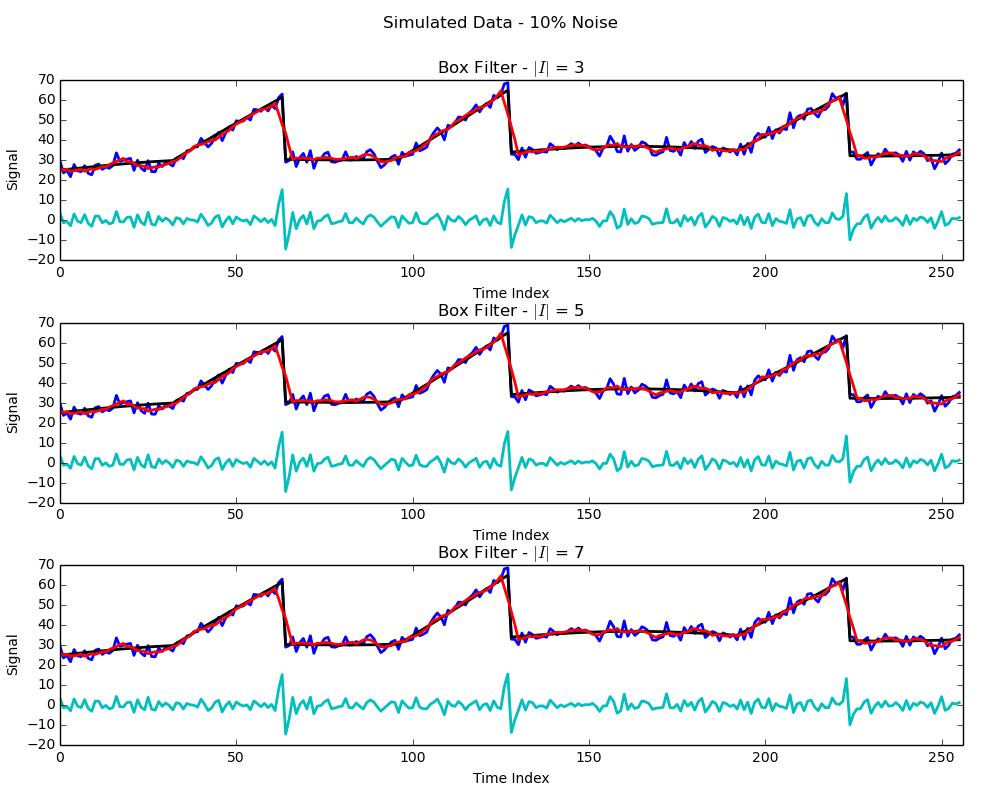
\includegraphics[width = 0.9 \textwidth]{BoxCompare.png}
\caption{Box Filter With Simulated Data}
\label{boxcompare}
\end{figure}

\FloatBarrier

%-------------------------------
\subsubsection{Gaussian filter} 
%-------------------------------
The Gaussian filter is a weighted moving average that weights points
based upon their distance from the point of interest according to a
Gaussian distribution with standard deviation $\sigma_d$. The smoothed
values from the Gaussian filter are given by

\begin{displaymath}
s_i = \sum _{j \in I} w \left(i, j \right) y_j
\end{displaymath}

\noindent
where the weights are given by the function

\begin{displaymath}
w\left(i, j\right) = \frac{1}{z_i} e^{-\frac{\lvert i - j \rvert}{2 \sigma_d^2}}
\end{displaymath}

\noindent
and $z_i$ is a normalization factor so the weights sum to $1$ on the interval.

Typically a interval width of $10 \sigma_d$ is used. This accounts for
$99.99994\%$ of the Gaussian distribution. Some computations can be
saved by using an interval width of $8 \sigma_d$, $99.994\%$ of the
Gaussian distribution, or $6 \sigma_d$, $99.7\%$ of the Gaussian
distribution. In this technique, the Gaussian kernel standard
deviation, $\sigma_d$, is a parameter to be chosen by the analyst.
Figure \ref{gaussiandemo} shows the weighting scheme for the Gaussian
filter.

\begin{figure}[h!]
\centering
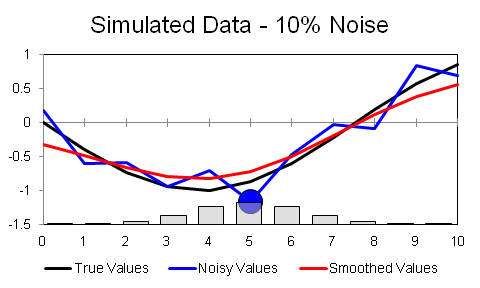
\includegraphics[width = 0.4 \textwidth]{GaussianDemo.png}
\caption{Gaussian Filter Weighting Scheme}
\label{gaussiandemo}
\end{figure}

As seen in Figure \ref{gaussiancompare}, the Gaussian filter does a
reasonable job removing noise but also destroys features in the time
series, albeit to a lesser degree than for a box filter with the same
window size. The damage to the three jumps can again be seen in the
residuals, show in cyan in the figure.

\begin{figure}[h!]
\centering
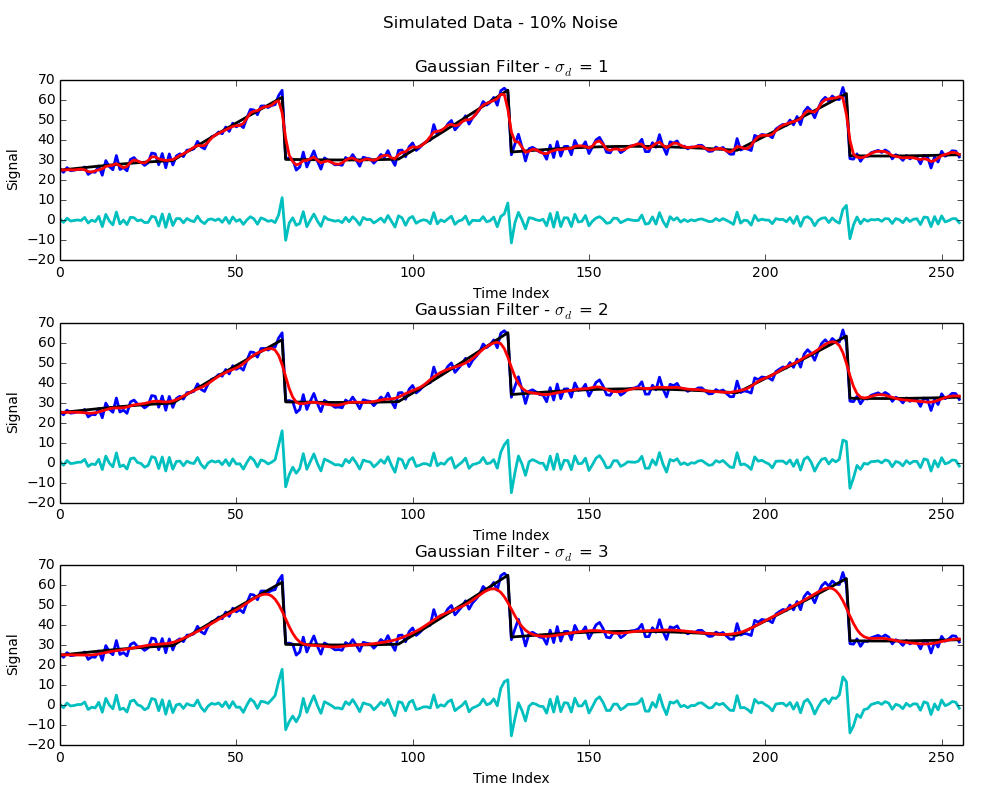
\includegraphics[width = 0.9 \textwidth]{GaussianCompare.png}
\caption{Gaussian Filter with Simulated Data}
\label{gaussiancompare}
\end{figure}

\FloatBarrier


%--------------------------------
\subsubsection{Bilateral filter} 
%--------------------------------
The bilateral filter~\cite{tomasi98:bilateral} attempts to better
preserve features in the time series by applying a pair of Gaussian
weights, one for spatial distance, as in the Gaussian filter, and one
for differences in intensity values. The smoothed values from the
bilateral filter are given by

\begin{displaymath}
s_i = \sum _{j \in I} w \left(i, j \right) y_j
\end{displaymath}

\noindent
where the weights are given by the function

\begin{displaymath}
w\left(i, j\right) = \frac{1}{z_i} e^{-\frac{\lvert i - j \rvert}{2 \sigma_d^2}}e^{-\frac{\lvert y_i - y_j \rvert}{2 \sigma_i^2}}
\end{displaymath}

\noindent
and, as before, $z_i$ is a normalization factor.

As with the Gaussian filter, an interval width of $10 \sigma$ is typical. In this
technique, the Gaussian kernel standard deviations, $\sigma_d$ and
$\sigma_i$, are two parameters to be chosen by the analyst. Figure
\ref{bilateraldemo} shows the weighting scheme for the bilateral
filter.

\begin{figure}[h!]
\centering
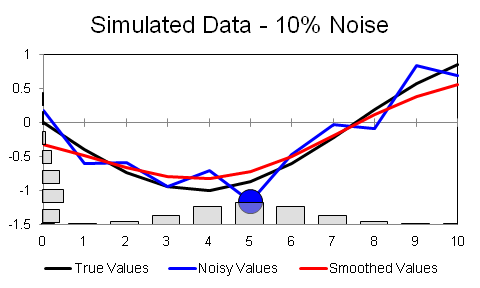
\includegraphics[width = 0.4 \textwidth]{BilateralDemo.png}
\caption{Bilateral Filter Weighting Scheme}
\label{bilateraldemo}
\end{figure}

As seen in Figure \ref{bilateralcompare}, the bilateral filter does a
reasonable job both smoothing the time series and retaining features.
Damage to the three jumps cannot be seen in the residuals.
Unfortunately, the bilateral filter may retain some of the noise,
particularly if the noise causes a significant change in intensity
value.

\begin{figure}[h!]
\centering
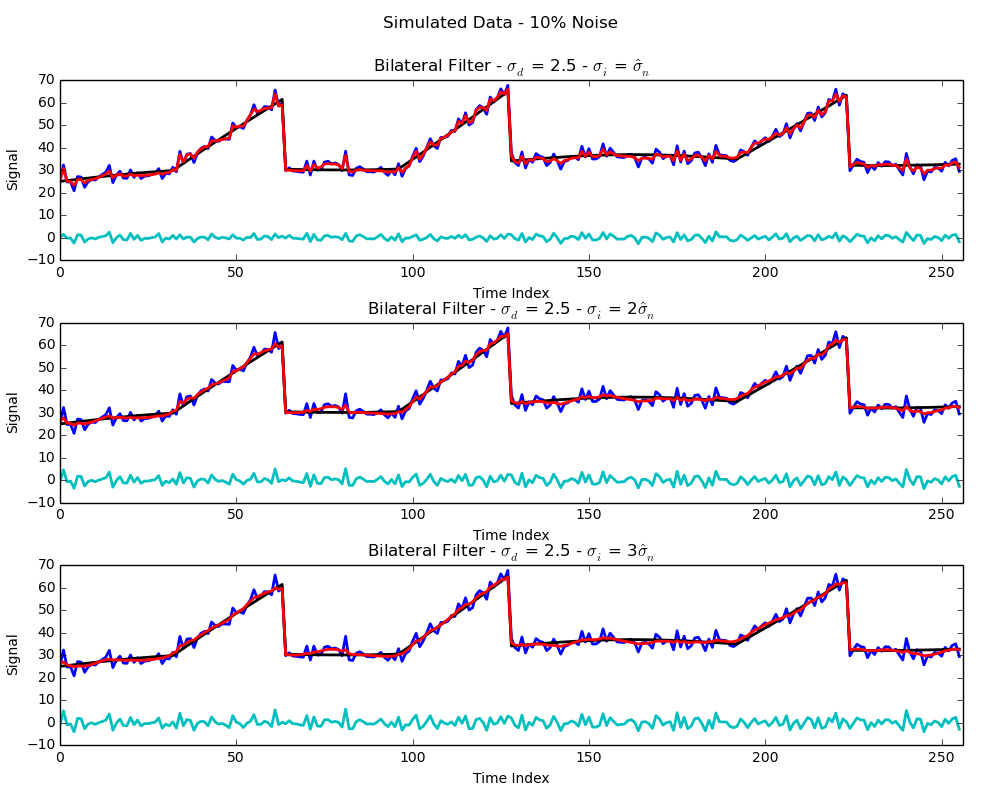
\includegraphics[width = 0.9 \textwidth]{BilateralCompare.png}
\caption{Bilateral Filter with Simulated Data}
\label{bilateralcompare}
\end{figure}

Zang and Gunturk~\cite{Zang08} suggest that the optimal value of the
standard deviation of the spatial Gaussian kernel, $\sigma_d$, is in
the range $\left[ 1.5, 2.1 \right]$ and the standard deviation of the
intensity Gaussian kernel, $\sigma_i$, is in the range $\left[ 1.5
  \hat{\sigma}_n, 3 \hat{\sigma}_n \right]$ for $2$D image processing. Recall that $\hat{\sigma}_n$ is the noise standard deviation estimate. It is
uncertain if these results translate to $1$D time series denoising.

\FloatBarrier


%-----------------------------------------------------------
\subsubsection{Treatment of edge values in spatial filters} 
%-----------------------------------------------------------

It is important to note that treatment of edge values is particularly
important when incrementally processing a time series as the most
relevant data is in the leading edge of the data set. In the case of
spatial filters, the $\frac{\lvert I \rvert - 1}{2}$ values on each
edge do not have complete intervals. We adjust normalization factor
$z_i$ to ensure that the weight values in the incomplete interval
still sum to $1$. Figure \ref{increment} shows the adjusted weighting
scheme for the box filter for the most recent data point, highlighted
in blue.

With this edge treatment, it is simple to adjust the time series when
a new data point is received. With the updated time series, the last
$\frac{\lvert I \rvert - 1}{2}$ smoothed values can be updated and a
new smoothed value can be calculated as before. Figure \ref{increment}
also highlights the updated values, in red. These comments on edge
treatment and incrementing also apply to our implementation of the
other spatial filters, namely the Gaussian and bilateral filters.

\begin{figure}[h!]
\centering
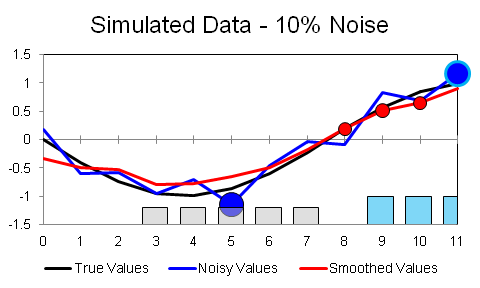
\includegraphics[width = 0.4 \textwidth]{Increment.png}
\caption{Updated Edge Values for Local Smoothing Filters}
\label{increment}
\end{figure}



%=================================
\subsection{Frequency techniques}
%=================================
%----------------------------------
\subsubsection{Fourier transform} 
%----------------------------------
Historically, analysis in the frequency domain was conducted via the
Fourier transform in its rapid discrete form, the Fast Fourier
Transform (FFT). The FFT takes uniformly spaced observations and can
transform the data relatively quickly. After transformation,
coefficient thresholding is used on the time series frequency
coefficients to denoise the data, and then the denoised frequency
coefficients are reverse transformed.

There are two common procedures for modifying noisy frequency
coefficients, known as thresholding methods~\cite{Donoho94}. The
first, hard thresholding, cancels all coefficients smaller than a
particular threshold. $v\left(\alpha\right)$ represents the frequency
coefficients of the time series, the result of transforming data. In
hard thresholding, the denoised coefficients are given by:

\begin{displaymath}
v\left(\alpha\right) = 
\begin{cases}
v\left(\alpha\right) & \lvert v\left(\alpha\right)\rvert > \mu \\
0 & \lvert v\left(\alpha\right)\rvert < \mu
\end{cases}
\end{displaymath}

Hard thresholding can create outliers, which can be partially avoided
using soft thresholding. In soft thresholding the denoised
coefficients are given by:

\begin{displaymath}
v\left(\alpha\right) = 
\begin{cases}
v\left(\alpha\right) - sgn\left(v\left(\alpha\right)\right)\mu & \lvert v\left(\alpha\right)\rvert \geq \mu \\
0 & \lvert v\left(\alpha\right)\rvert < \mu
\end{cases}
\end{displaymath}

Unfortunately, soft thresholding can create problems with the scale of
the reverse transformed data which can make it inappropriate for time
series where the scale of the data is important. For this reason, we
will only consider hard thresholding. In this algorithm, the analyst
can control the choice of hard or soft thresholding and the
thresholding cutoff, $\mu$.

The theoretically optimal threshold is $\mu = \sigma \sqrt{2 \log I}$,
where $I$ is the number of data points and $\sigma$ is the standard
deviation of the coefficients. In order to avoid inflating the
standard deviation of the coefficients through a large coefficient
corresponding to the mean of the data, the mean is subtracted from the
time series prior to transformation, making the time series a
zero-mean dataset. In practice this threshold is too high and cancels
too many coefficients that do not correspond to noise. Instead, $\mu =
3 \sigma$ is used for hard thresholding and $\mu = \frac{3}{2} \sigma$
is used for soft thresholding~\cite{Buades05} for $2$D image
processing. It is uncertain if these results translate to $1$D time
series denoising.

As can be seen in Figure \ref{fftcompare}, the Fourier transform
struggles near the edges, where Gibbs phenomenon may occur. This makes
the Fourier transform less than ideal for incremental data denoising,
where the most relevant data is near the end of the time series.

\begin{figure}[h!]
\centering
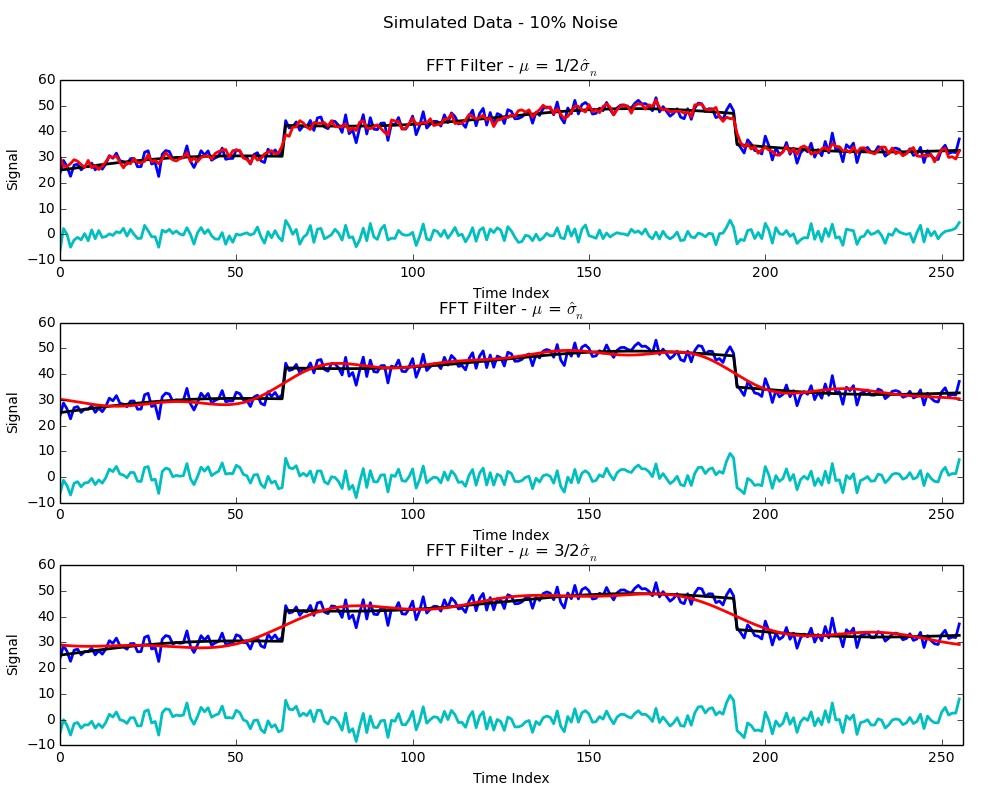
\includegraphics[width = 0.9 \textwidth]{FFTCompare.png}
\caption{Fourier Transform Filter with Simulated Data}
\label{fftcompare}
\end{figure}

Incremental updates present a problem for the Fourier transform, as
the transform can only be applied to multiple data points, and larger data sets are better. This means that it takes more
computations to incrementally update Fourier transform coefficient
thresholding smoothed time series than locally smoothed time series.

%---------------------------------
\subsubsection{Wavelet transform} 
%---------------------------------
The wavelet transform is one of the most popular frequency domain
alternatives to the Fourier transform. While the Fourier transform
completely transforms the time series into the frequency domain, the
wavelet transform offers both frequency and time information by
fitting a series of finite length functions, wavelets, to the time
series. One such wavelet is the Haar wavelet, Figure
\ref{haarwavelet}. This allows for filtering both by frequency and
temporal relationships~\cite{Graps95}. There are a variety of wavelet
families to choose from, and the wavelet transformations can be
repeated to a desired level of resolution. We use the Haar wavelet due
to its simplicity, but many other families of wavelets give better
performance.

\begin{figure}[h!]
\centering
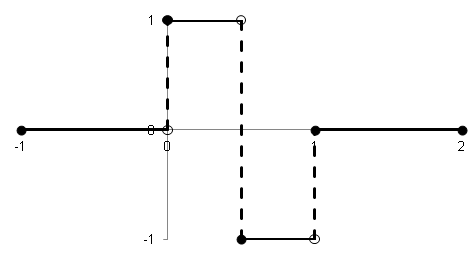
\includegraphics[width = 0.6 \textwidth]{HaarWavelet.png}
\caption{Haar Wavelet}
\label{haarwavelet}
\end{figure}

Mota, Vasconcelos, and Silva~\cite{Mota05} outlined a algorithm for
processing continuous data streams in real time using the discrete
wavelet transform, inspired by an older result by Vishwanath, called
the Recursive Pyramid Algorithm~\cite{Vishwanath94}.

Once the data has been wavelet transformed, the data is denoised via
frequency coefficient thresholding, as with the Fourier
transform~\cite{fodor03:denoising}.

In this technique, the analyst choses the wavelet family, the number
of levels of decomposition, and the thresholding cutoff, $\mu$. Figure
\ref{waveletcompare} shows the results from denoising with a Haar
wavelet transform, with different hard thresholds.

\begin{figure}[h!]
\centering
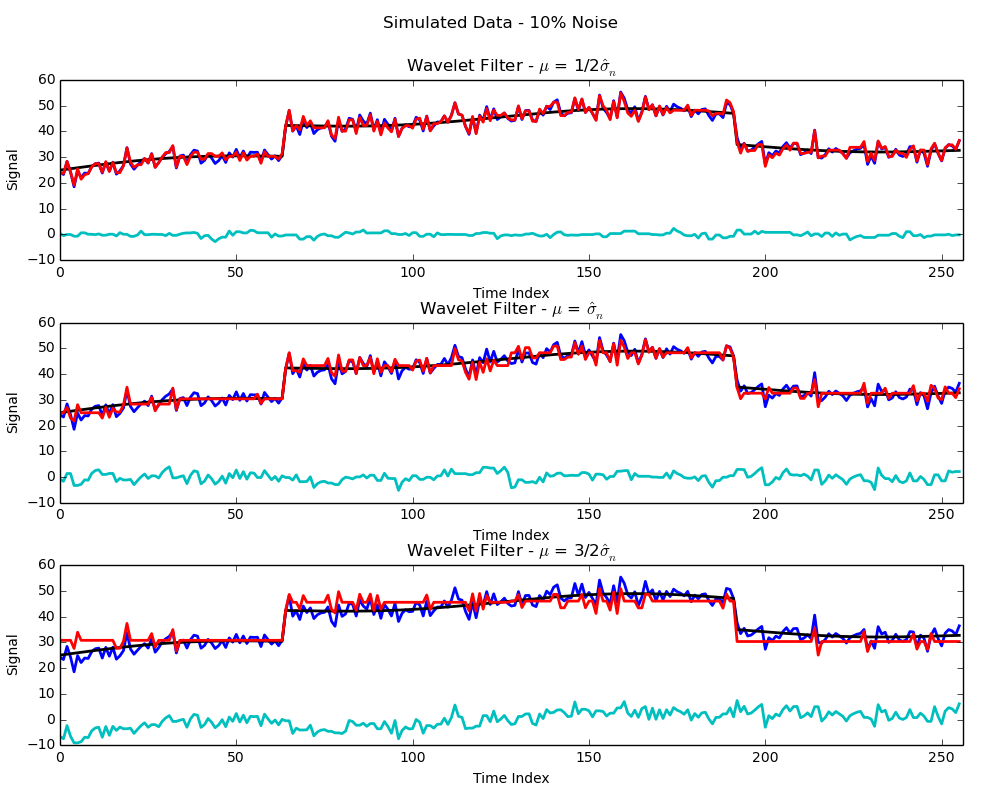
\includegraphics[width = 0.9 \textwidth]{WaveletCompare.png}
\caption{Wavelet Transform Filter with Simulated Data}
\label{waveletcompare}
\end{figure}

In this case, there is no special edge treatment. Incremental data
processing is often accomplished via a real time algorithm, as
mentioned above and frequency coefficients are thresholded and back
transformed immediately afterwards.

%============================================
\subsection{Statistical neighborhood filters}
%============================================
%------------------------------------------
\subsubsection{The non-local means algorithm} 
%------------------------------------------
Statistical neighborhood filters attempt to fix the problems
associated with local smoothing filters by calculating the smoothed
value as a weighted average of other values in the time series based
upon the similarity between the neighborhoods around the time series
values. Figure \ref{nlmeansdemo} shows three neighborhoods highlighted
in the time series. The values in the green window are more similar to
the values in the black window than the values in the red window and,
thus, should be weighted higher.

The non-local means algorithm was first introduced by Buades et
al.~\cite{Buades05}. Non-local means has primarily been used for image
processing, but it has been mentioned in a $1$D context in several
papers (~\cite{Galiano13},~\cite{Tracey12},~\cite{Zoican10}). We use
a modification of this algorithm for efficient $3$D medical image
processing by Coup{\'e} et al.~\cite{Coupe07}.

\begin{figure}
\centering
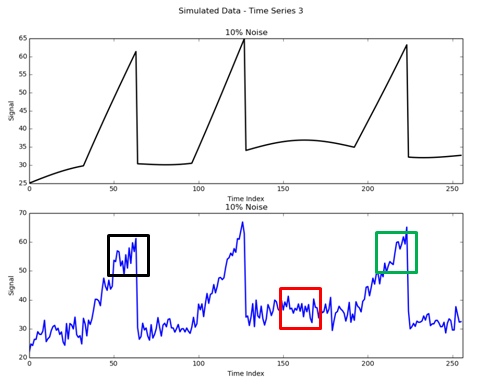
\includegraphics[width = 0.65 \textwidth]{NLMeansDemo.png}
\caption{Non-local Means Window Comparison}
\label{nlmeansdemo}
\end{figure}

In the non-local means algorithm, smoothed values are given by

\begin{displaymath}
s_i = \sum _{j \in N} w \left(i, j \right) y_j
\end{displaymath}

\noindent
where the weights are given by the function

\begin{displaymath}
w \left(i, j \right) = \frac{1}{z_i} e^{-\frac{\lvert Y_i - Y_j \rvert ^2}{2 \beta \hat{\sigma}^2_n \lvert Y \rvert}}
\end{displaymath}

In this scheme, $Y_i$ is a vector of intensity values in the window,
or neighborhood, around $y_i$, $\lvert Y_i - Y_j \rvert$ is the $L_2$
norm of the difference in intensity values in these intervals, $\lvert
Y \rvert$ is the window size, and $\beta$ is a parameter chosen by the
analyst to control the amount of smoothing. According to Coup{\'e} et
al.~\cite{Coupe07}, $\beta$ varies between $0.0$ and $1.0$, with
values of $\beta$ closer to $1.0$ better for high levels of noise and
values of $\beta$ closer to $0.5$ better for lower levels of noise.

Duval et al.~\cite{Duval11} notes that neighborhood preselection can
improve the results of the non-local means algorithm by assigning a
weight of $0$ to the $y_j$ values that have neighborhoods that are too
dissimilar to the neighborhood, $Y_i$, under consideration. Duval et
al. uses a preselection test based upon the norm of the difference
between neighborhoods. A more complex preselection method is described
by Buades et al.~\cite{Buades05}. We use Duval et al.'s preselection
test:

\begin{displaymath}
w\left(i, j\right) = 
\begin{cases}
\frac{1}{z_i} e^{-\frac{\lvert Y_i - Y_j \rvert ^2}{2 \beta \hat{\sigma}^2_n \lvert Y \rvert}} & \lvert Y_i - Y_j \rvert < T \\
0 & $otherwise$
\end{cases}
\end{displaymath}

Duval et al.~\cite{Duval11} suggests that values of $T$ near $20$ or
$30$ work well for $2$D images. This threshold does make sense for
denosing time series. We will consider thresholds of the type $T =
\delta \left( \mathrm{max} Y_j - \mathrm{min} Y_j \right) \lvert Y
\rvert$, where $\delta \in \left[ 0.0, 1.0 \right]$. This threshold is
a percentage of an approximation of the maximum intensity interval
distance. Duval et al. recommends window sizes of $5$ or $7$ for $2$D
image processing. As before, it is uncertain if these results
translate to $1$D time series denoising.

In this algorithm, the analyst can control the amount of smoothing via
$\beta$, the preselection parameter $\delta$, the window size, and the
portion of the time series that is compared. Figure
\ref{nlmeanscompare} shows the performance of the non-local means
algorithm with different values of $\beta$. Notice how similar the
performance is to the bilateral filter, Figure \ref{bilateralcompare}.

\begin{figure}[h!]
\centering
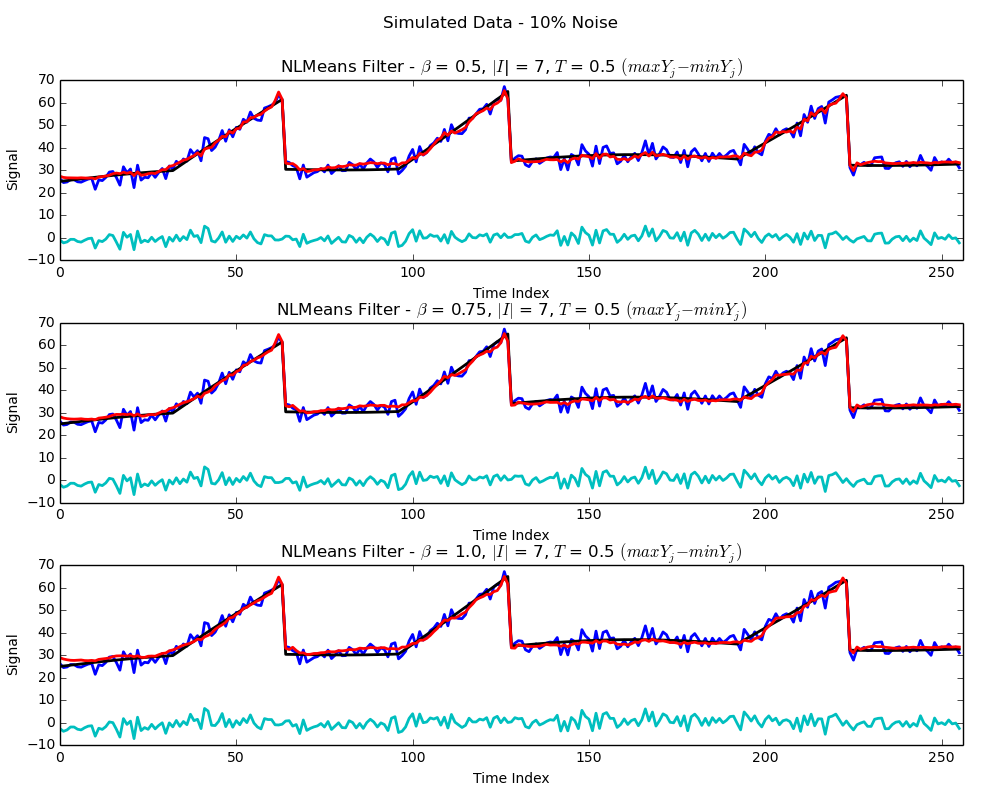
\includegraphics[width = 0.9 \textwidth]{NLMeansCompare.png}
\caption{Non-Local Means with Simulated Data}
\label{nlmeanscompare}
\end{figure}

As with the spatial filters, the $\frac{\lvert I \rvert - 1}{2}$
values on the edges do not have complete intervals, or windows. In
order to calculate weights, we compare the incomplete neighborhood
$Y_i$ with incomplete neighborhoods around the other points $Y_j$. We
adjust normalization factor $z_i$ to ensure that the weight values in
the incomplete interval still sum to $1$.

With this edge treatment, it is simple to adjust the time series when
a new data point is received. With the updated time series, the last
$\frac{\lvert I \rvert - 1}{2}$ smoothed values can be updated and a
new smoothed value can be calculated as before.


\FloatBarrier

%====================================
\subsection{Combination approaches} 
%====================================

An obvious question to ask is the following: can we do better by
combining denoising techniques, that is, applying them in succession
to the data? A motivation for this is the non-local means algorithm,
where we might expect to find better matches if the data was denoised
first.

Iterating the box filter and Gaussian filter is well understood
and is equivalent to using a box filter with a
wider interval or Gaussian filter with a larger kernel, $\sigma_d$. We do not investigate
these here. Iterating the Fourier transform or wavelet transform
coefficient thresholding is equivalent to using a Fourier transform or
wavelet transform filter with a higher frequency coefficient
threshold. We do will not investigate these here either. We also do
not consider combinations of frequency and spatial or statistical
neighborhood techniques, as these have been investigated elsewhere.

Iterating a bilateral filter or non-local means filter is more
complex. Also, the question of combining a bilateral filter and
non-local means filter is open. We will investigate all three of these
possibilities.

%========================================================
\section{Design of experiments for empirical comparison}
\label{design}
%=======================================================

The denoising techniques described in Section \ref{denoise} are
evaluated using peak signal to noise ratio (PSNR), for known time
series with added noise. 
%
%===================================
%\subsection{Evaluation methodology} 
%===================================
%
PSNR~\cite{Thu08} is the ratio between the maximum possible value of a time series and the maximum value of the noise. It is a measure of how noisy a signal
is, and therefore how effective a denoising algorithm was and is calculated as follows:

\begin{displaymath}
PSNR = 10 \cdot \log _{10} \left( \frac{ \left(\max\limits_{i} \{y_i\} \right)^2}{MSE} \right)
\end{displaymath}

\noindent
where $MSE$, mean square error, is

\begin{displaymath}
MSE = \frac{1}{N} \sum _{i = 0} ^{N - 1} \left( y_i - s_i \right) ^2.
\end{displaymath}

% It is important to note that PSNR is one of the most popular, but
% not the only, measure of quality for a denoised time series. PSNR is
% a global measure of quality, where higher values indicate a less
% noisy signal. An ideal denoising method is relatively insensitive to
% parameter choice within an optimal range and provides the best
% increase in PSNR.

In real world data, we do not know the true time series values are in
most cases, otherwise there is no need to denoise. Hence, PSNR can not
be used to evaluate such data. Therefore, we create three synthetic
time series that contain features similar to those in real
world data. We select denoising parameters based on best PSNR values.
Then, we view the effect of these parameters on real world data.


%============================
\subsection{Real world data}
%============================

As an example of real world data, we consider the weather data from
weather stations near the wind farms in the Bonneville Power
Administration (BPA) balancing area. 
%
% We chose eight stations that have data from the same weather measurements. 
%
The data in the time series was sampled at 5 minute intervals. Each weather
station measures seven variables, as shown in 
%
% The names of these stations and the seven variables available at each
% location are listed in Table~\ref{tb:weather}.
Figure~\ref{fig:weather_oct2011}, for the Augspurger station on
October 10, 2011.

\begin{comment}
\begin{table}[h!]
  \begin{center}
%\scriptsize
  \begin{tabular}{l|l}
    \hline
	\textbf{Weather Station} & \textbf{Measurement} \\
	\hline
    Augspurger (A)   & barometric pressure  \\
    Biddle Butte (B) & relative humidity  \\
    Hood River (HR)  & temperature  \\
    Mt Hebo (MH)     & wind direction\\
    Roosevelt (R)    & wind speed\\
    Sunnyside (SS)   & peak speed\\
    Tillamook (Ti)   & peak direction\\
    Troutdale (Tr)   & \\
    \hline
  \end{tabular}
  \end{center}
  %\vspace{-0.2in}
  \caption{\small The names of the eight weather stations near the BPA balancing area. Each of the stations has seven weather measurements, resulting in 56 variables.}
\vspace{-0.2in}
\label{tb:weather}
\end{table}
\end{comment}

\begin{figure}[h!]
\begin{center}
\begin{tabular}{cccc}
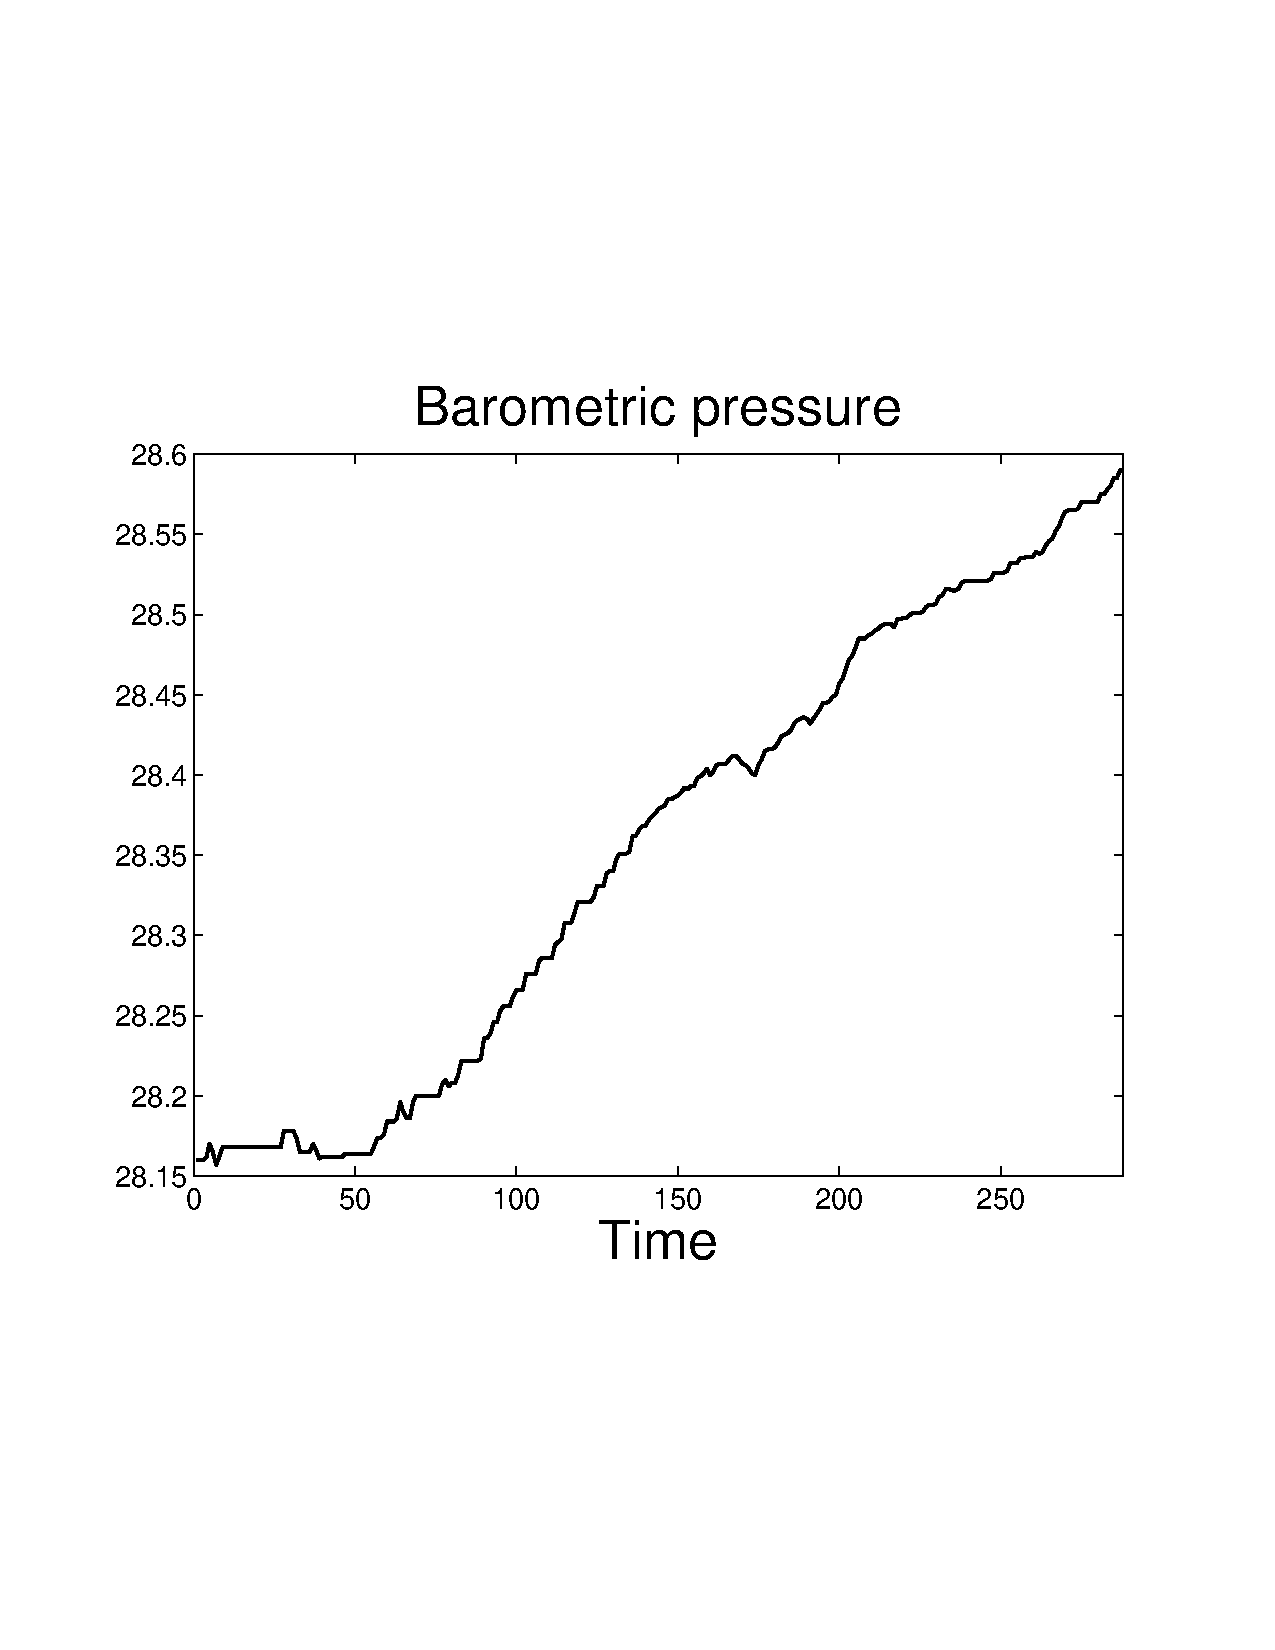
\includegraphics[trim=2.5cm 8cm 3cm 5cm,width=0.22\columnwidth]{201110_1day_B1.pdf} &
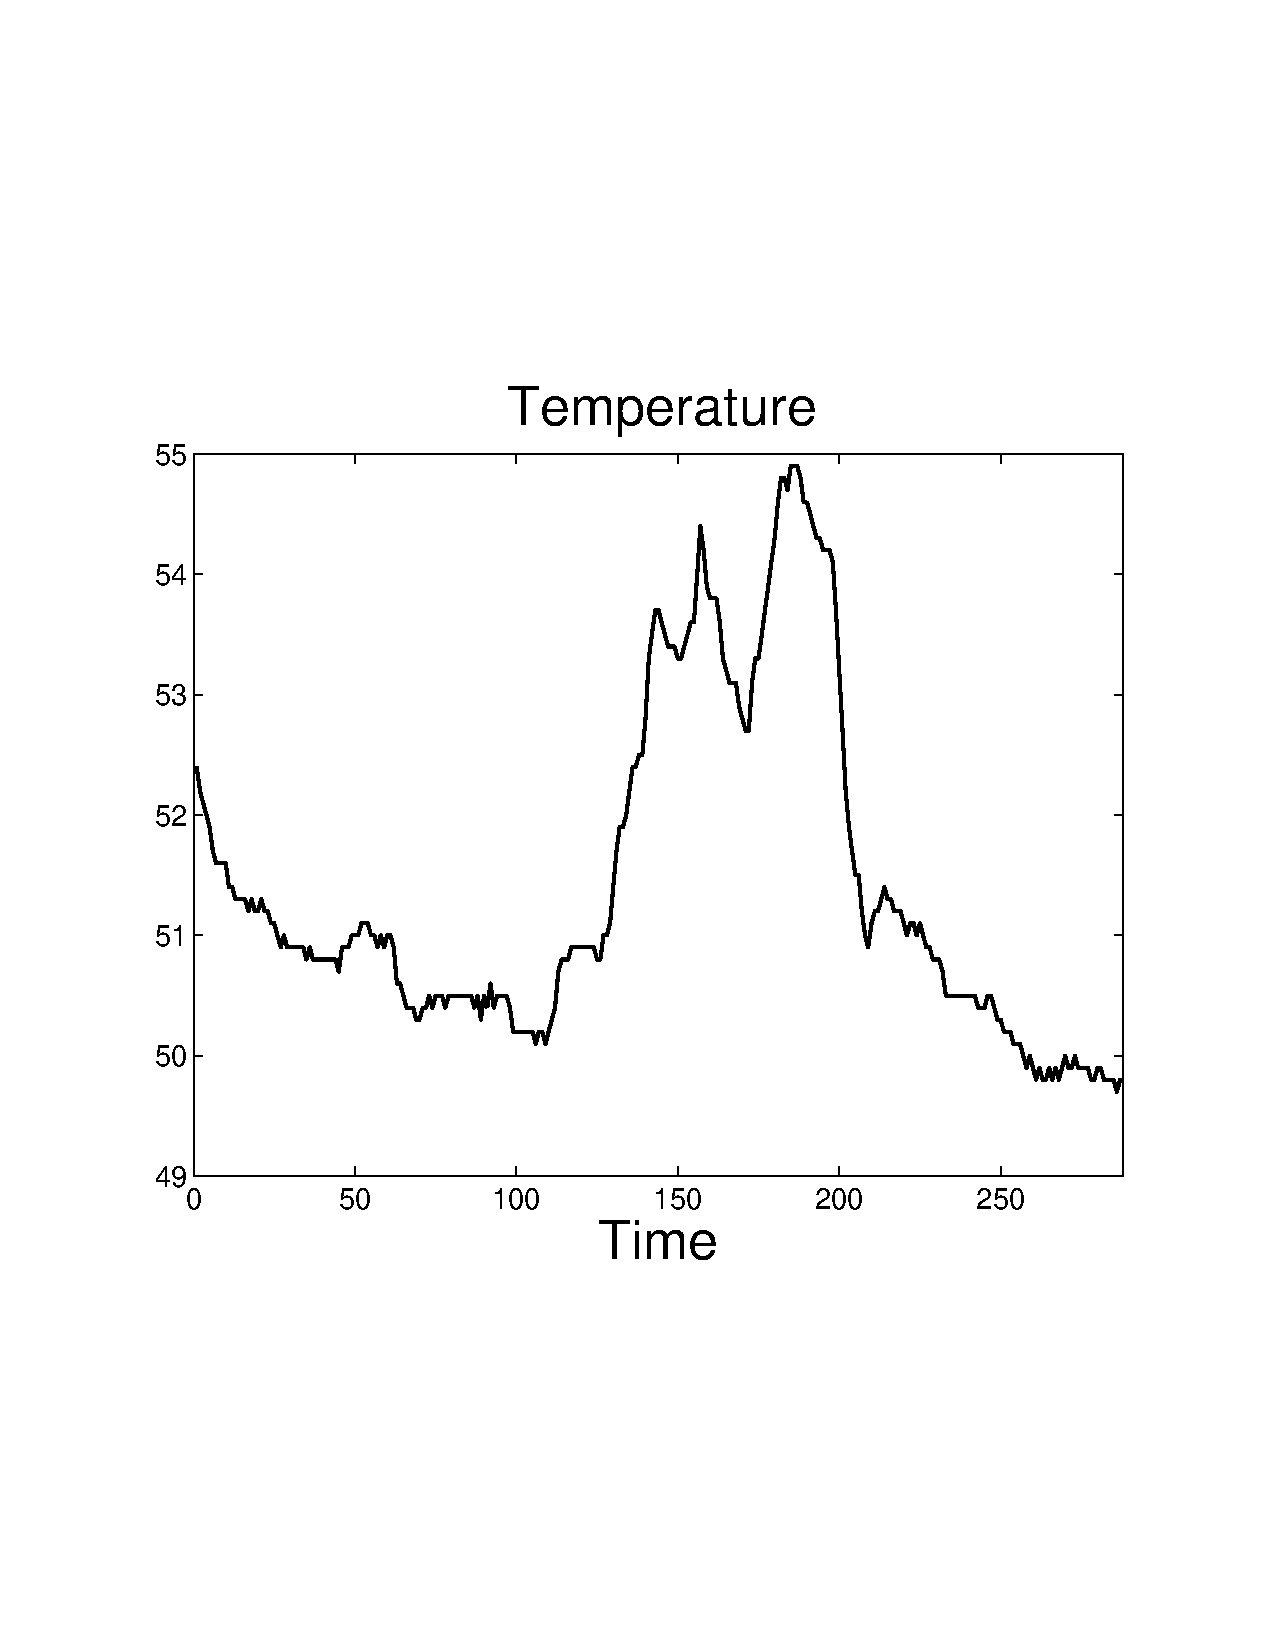
\includegraphics[trim=2.5cm 8cm 3cm 5cm,width=0.22\columnwidth]{201110_1day_B3.pdf} &
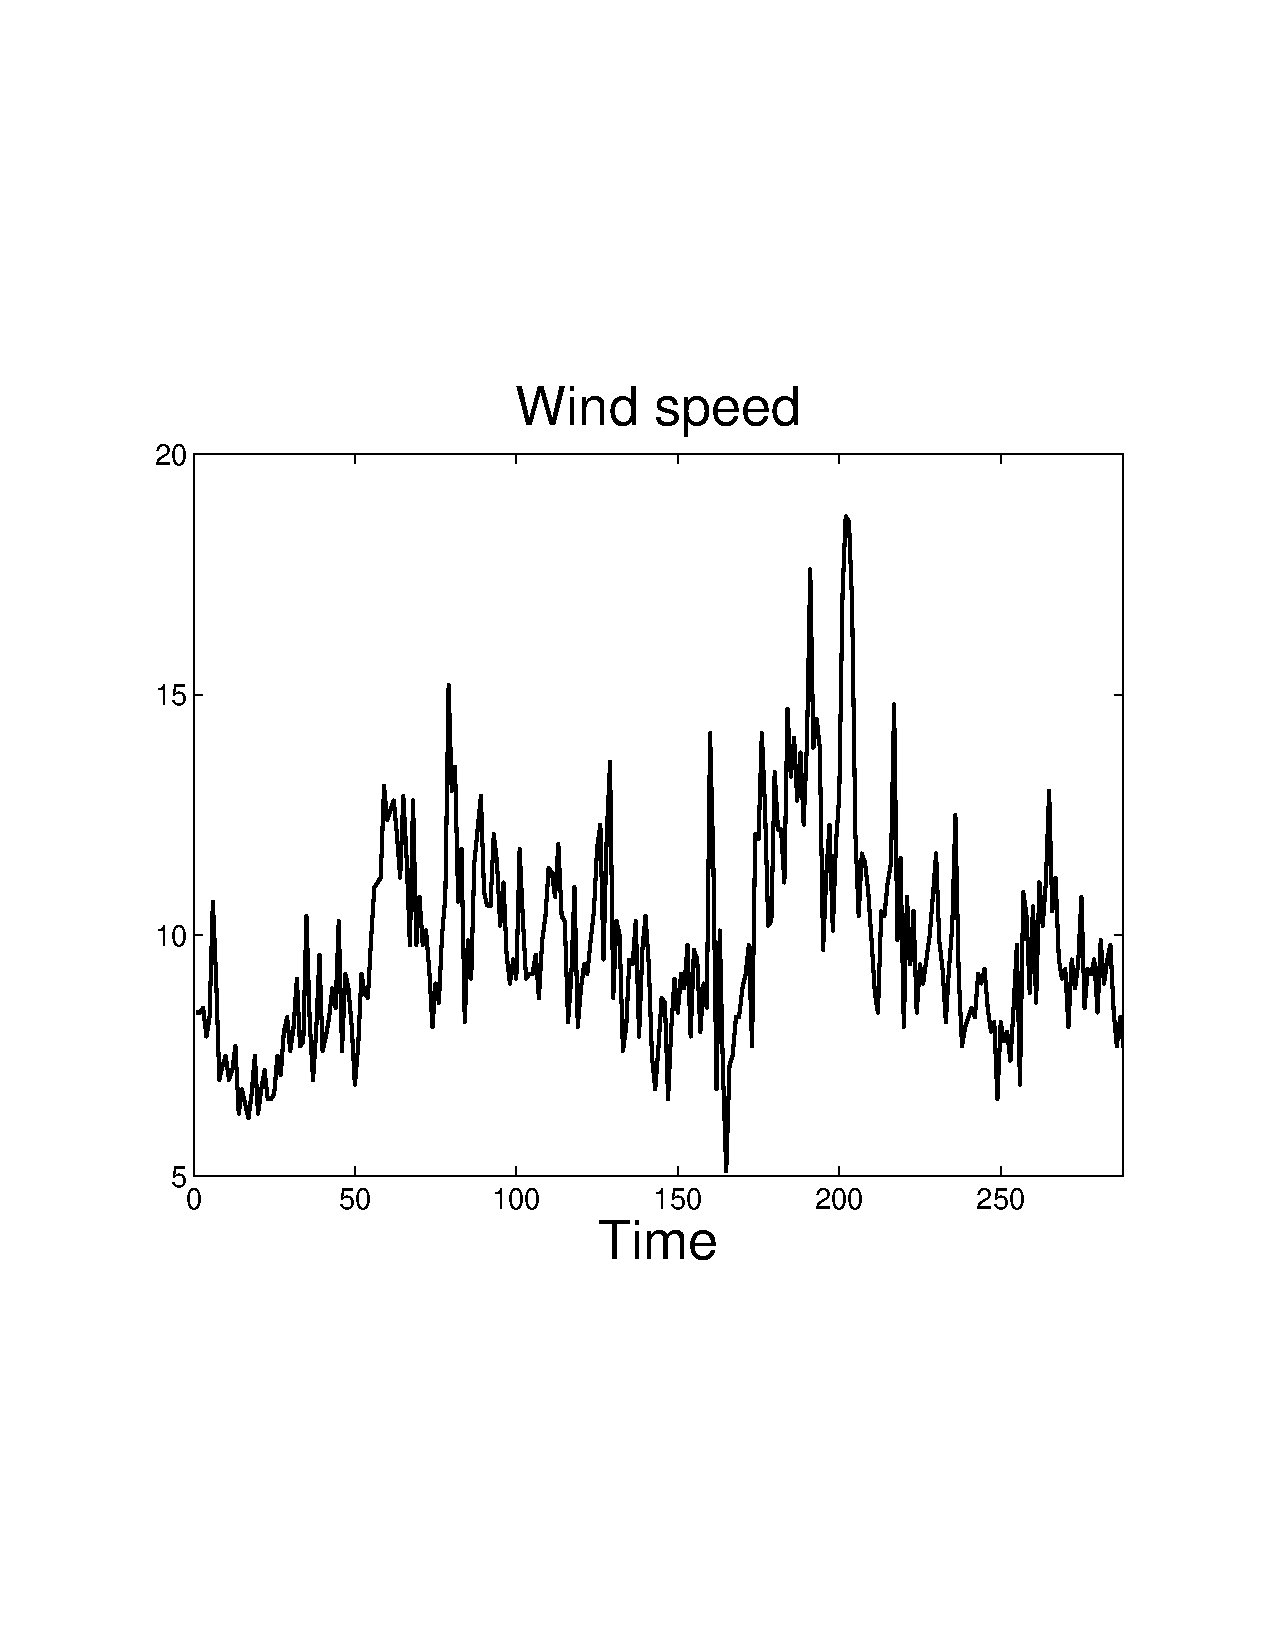
\includegraphics[trim=2.5cm 8cm 3cm 5cm,width=0.22\columnwidth]{201110_1day_B5.pdf} & 
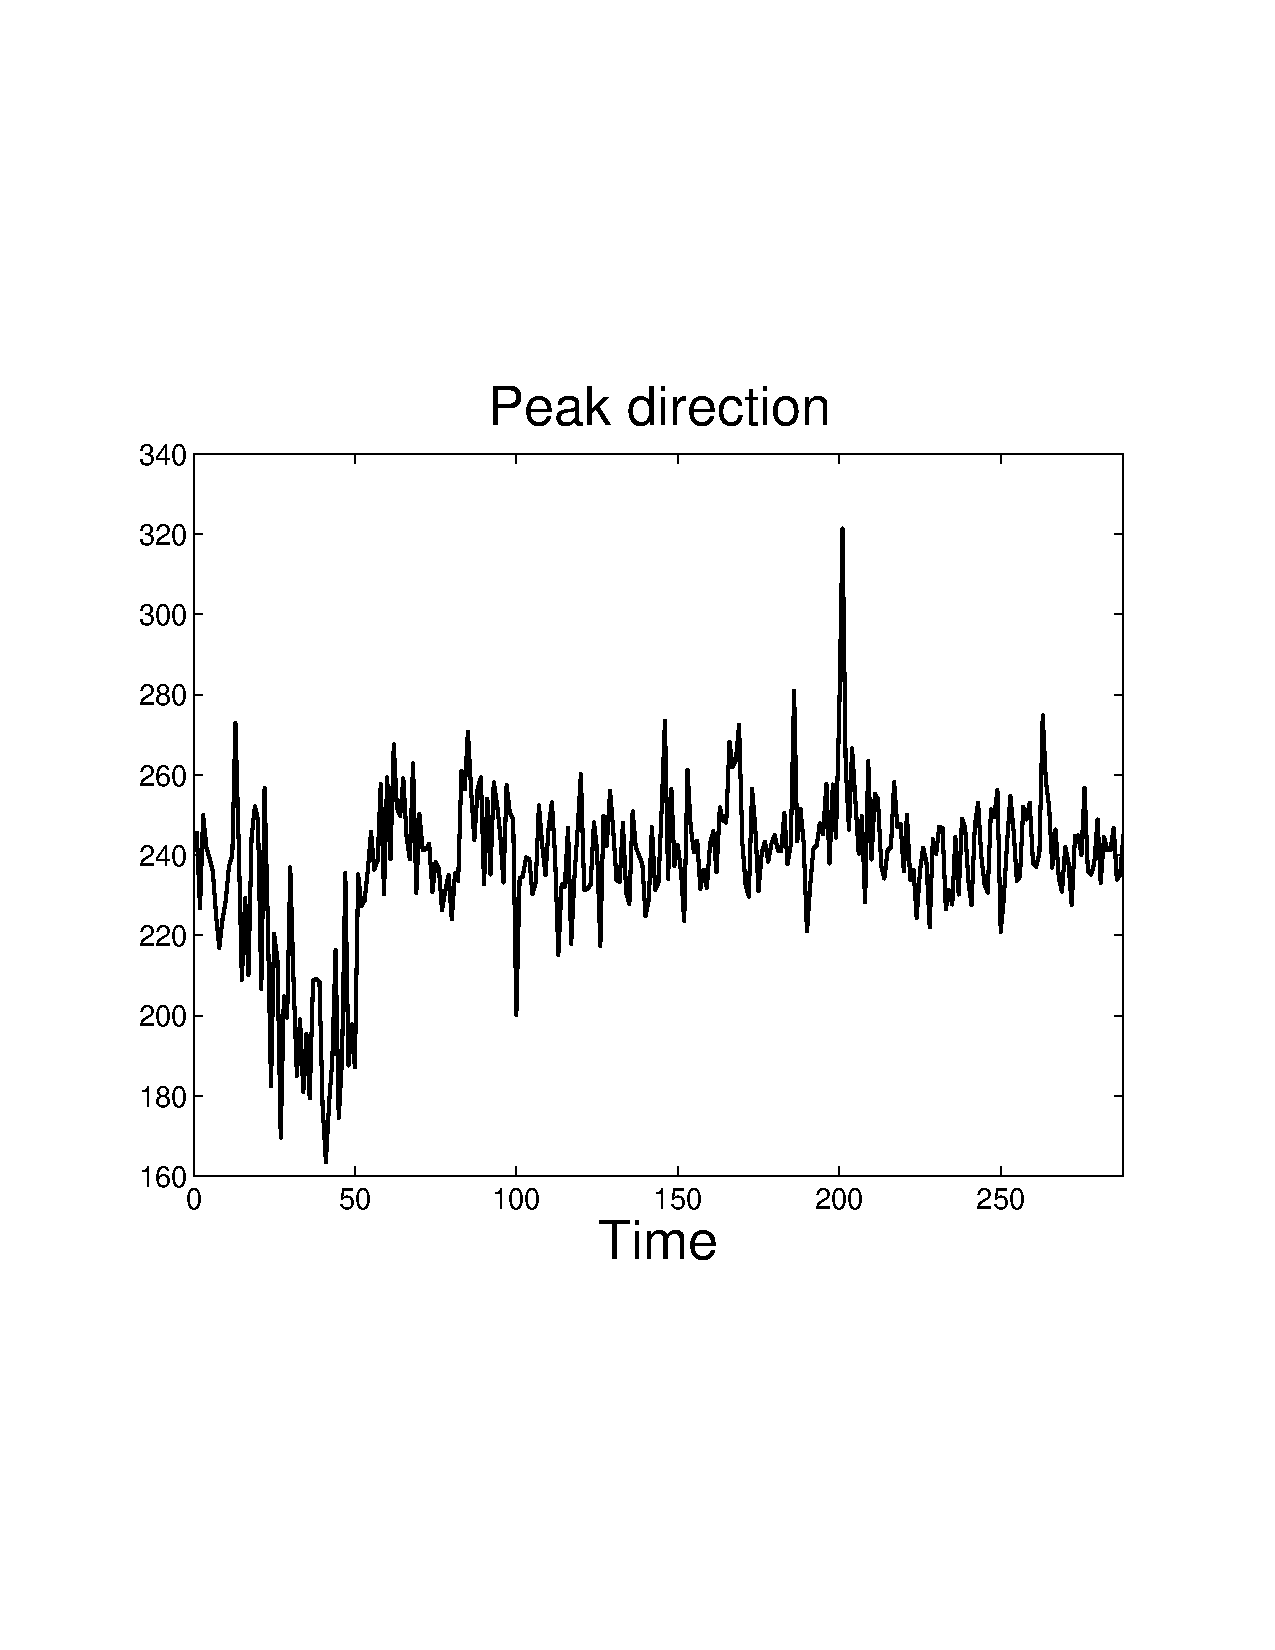
\includegraphics[trim=2.5cm 8cm 3cm 5cm,width=0.22\columnwidth]{201110_1day_B7.pdf} \\
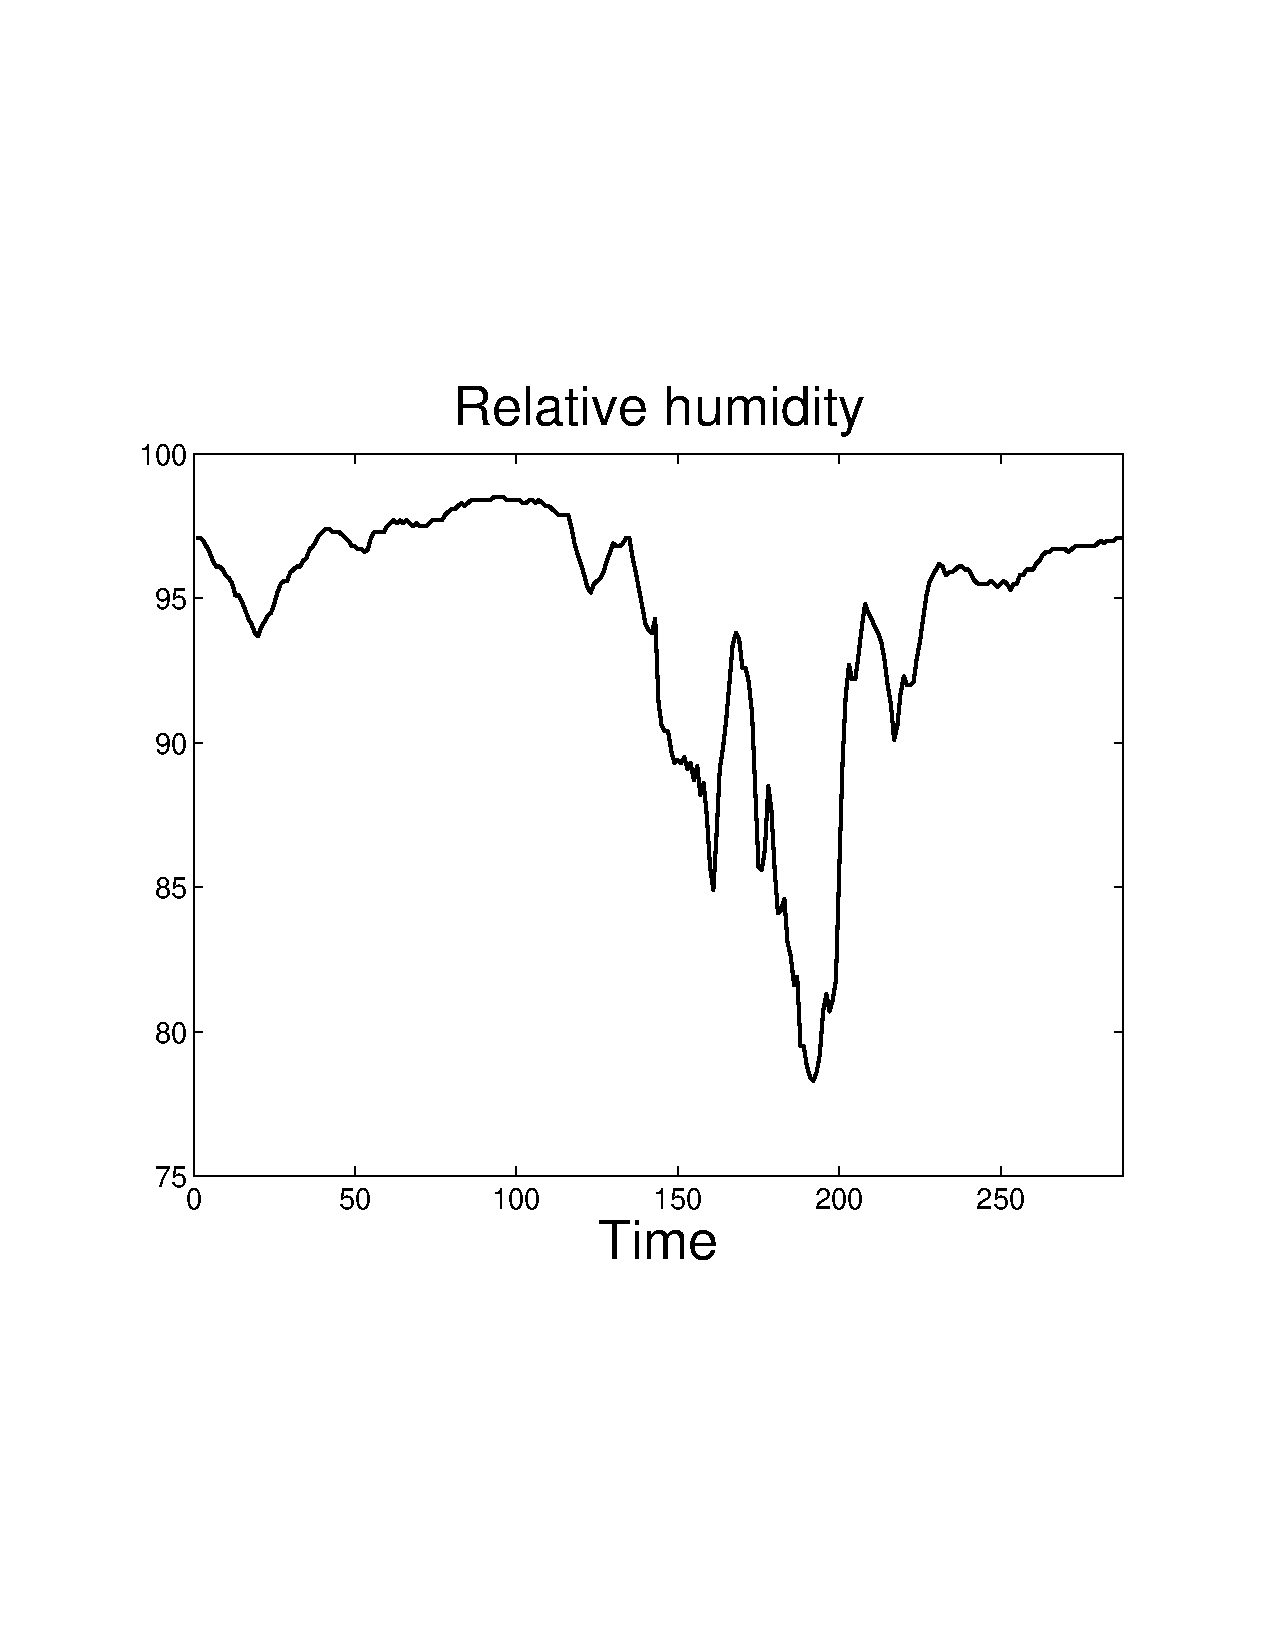
\includegraphics[trim=2.5cm 8cm 3cm 5cm,width=0.22\columnwidth]{201110_1day_B2.pdf} & 
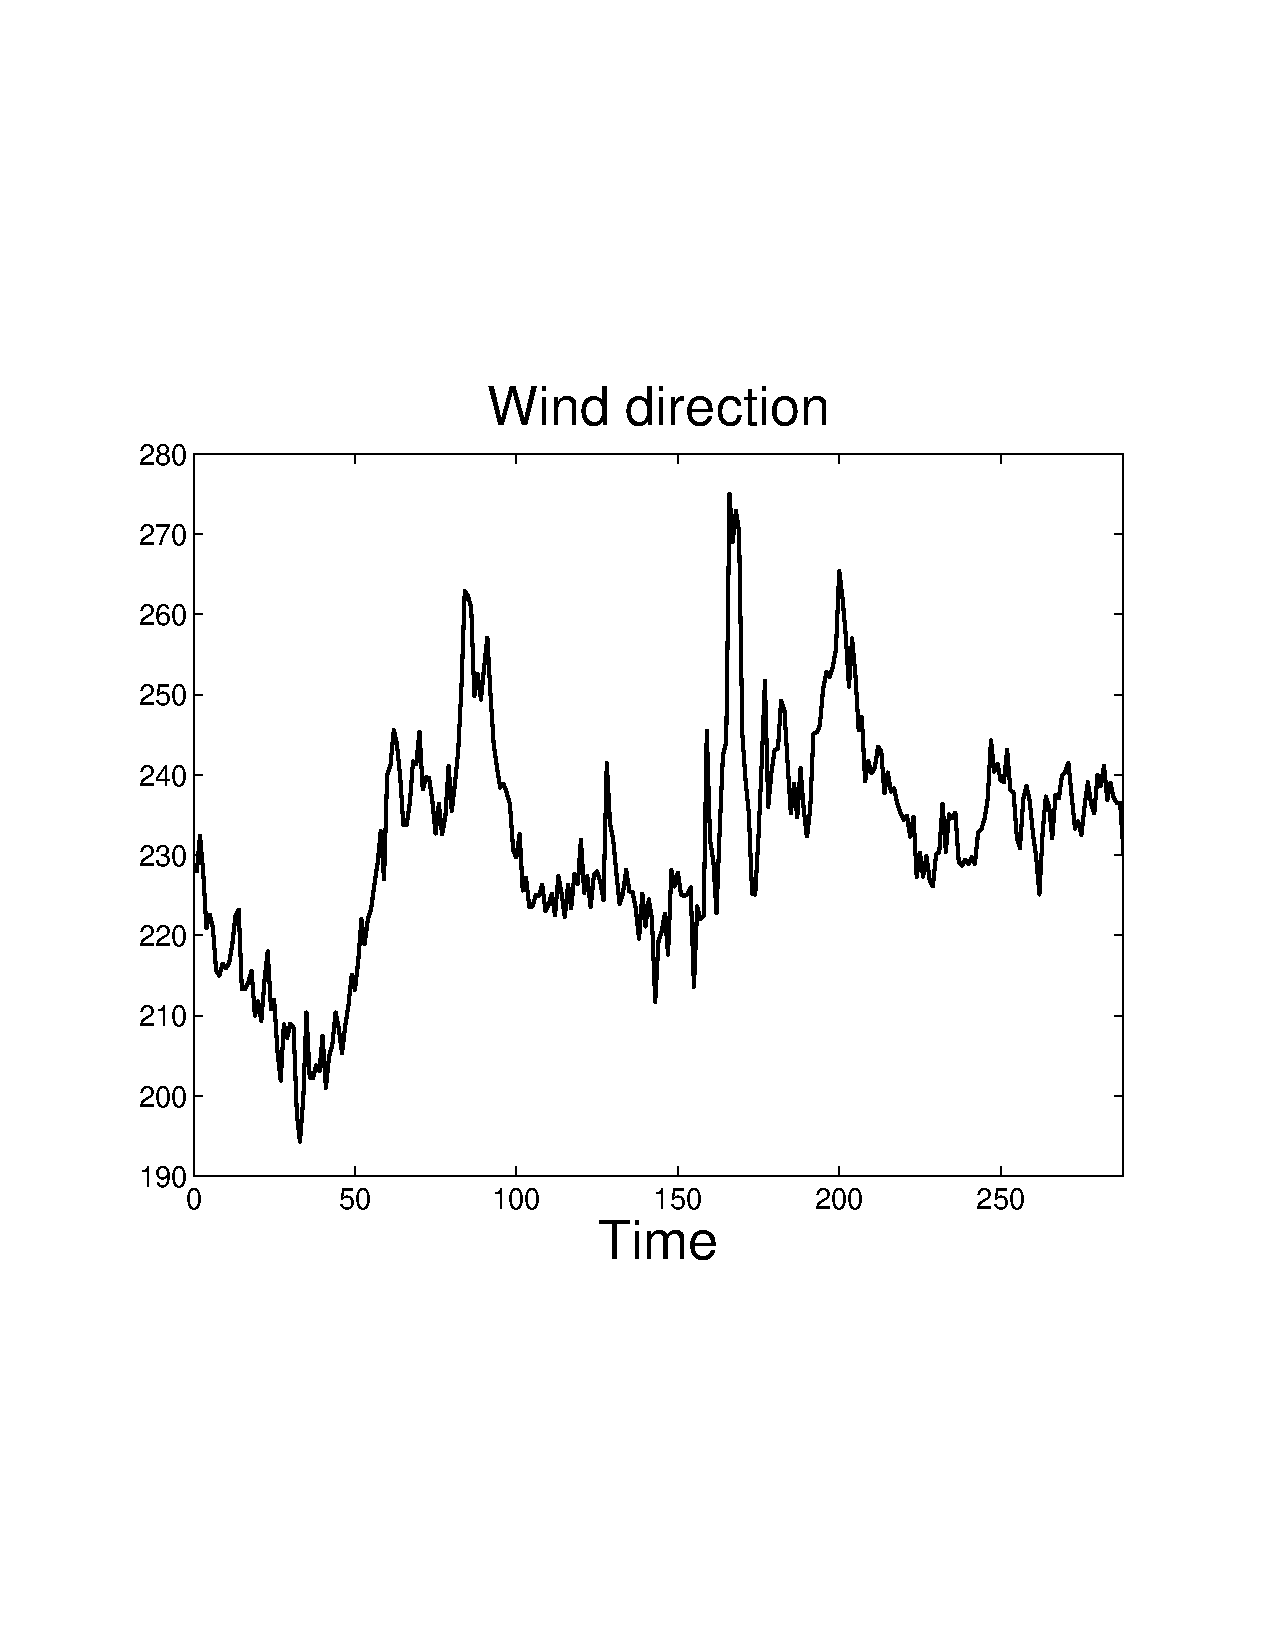
\includegraphics[trim=2.5cm 8cm 3cm 5cm,width=0.22\columnwidth]{201110_1day_B4.pdf} &
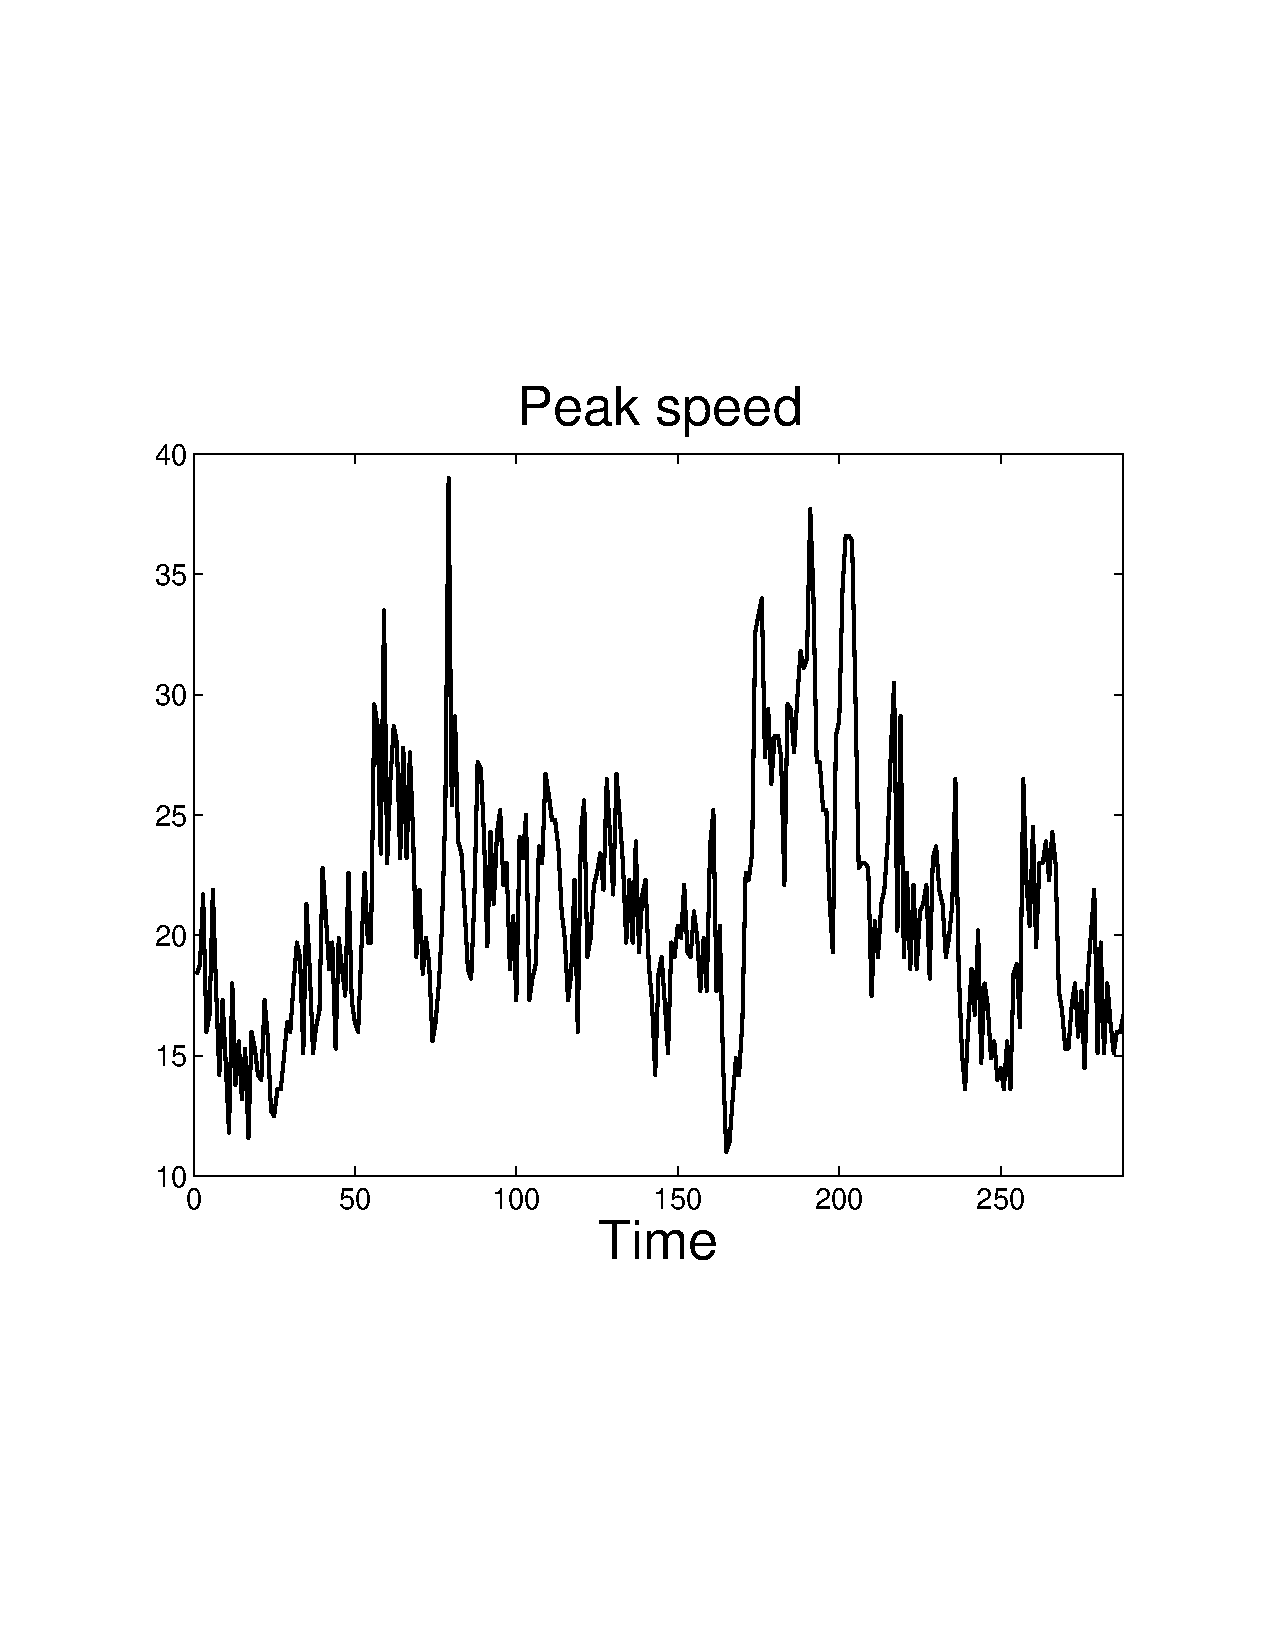
\includegraphics[trim=2.5cm 8cm 3cm 5cm,width=0.22\columnwidth]{201110_1day_B6.pdf} & \\
\end{tabular}
\end{center}
\vspace{-0.05in}
\caption{\small The Seven Weather Variables - Barometric Pressure,
  Temperature, Wind Speed, Peak Wind Speed, Wind Direction, Peak Wind
  Direction, and Relative Humidity - on October 10, 2011.}
\vspace{-0.15in}
\label{fig:weather_oct2011}
\end{figure}

%==============================
\subsection{Synthetic data} 
%==============================

One of the most popular noise models is Additive White Gaussian Noise
(AWGN). AWGN is comprised of independent identically
distributed real values from the Gaussian distribution with known, or
more commonly unknown, standard deviation, $\sigma_n$. 

Noise of a particular percentage is added by using $\sigma_n = p\cdot
v$ [? $2\sigma_n = p\cdot v$?] as the standard deviation of the
distribution that generated the noise, were $v =\max\{Y\} - \min\{Y\}$
is the maximum possible range of values that the time series $Y$ could
take and $0\leq p\leq 1$ is the percentage. To evaluate the
performance we apply denoising techniques on three known time series
with $ p = 1, 5, 10, 20$ and $30 \%$ AWGN noise added. Figure
\ref{signalscompare} displays the time series with $ p = 10\%$ noise
added.

\begin{figure}[h!]
\centering
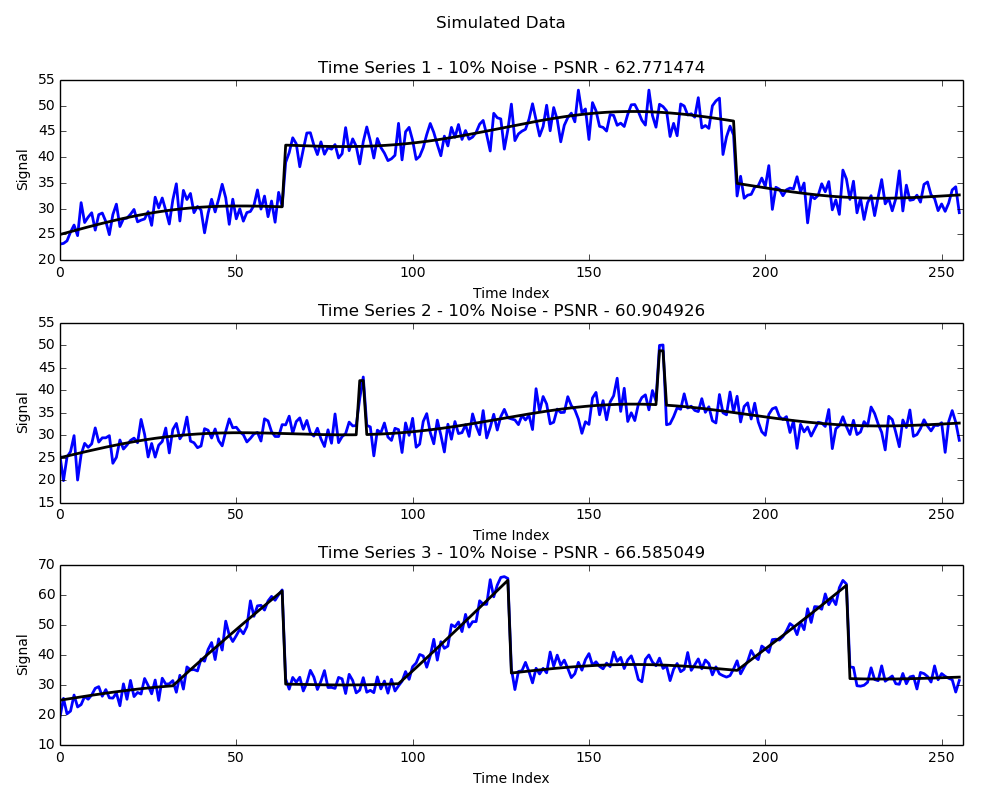
\includegraphics[width = 0.65 \textwidth]{SignalsCompare.png}
\caption{Known Time Series - 10\% Noise}
\label{signalscompare}
\end{figure}

All of the time series were created by taking low frequency sinusoidal
behavior and adding features of interest. There are a few interesting
observations that can be made about the three time series.

The first time series was created by taking low frequency sinusoidal
behavior and adding a sharp increase in intensity one quarter of the
way through the time series and adding a sharp decrease in intensity
three quarters of the way through the time series. In some cases the
noise obscures the sharp increase or decrease in intensity, making it
appear to be a more gradual increase or decrease in intensity. Noise
can make features impossible to recover. 

The second time series was created by taking low frequency sinusoidal
behavior and adding two brief, sharp increases in intensity, at one
and two thirds of the way through the time series. In some cases the
noise can become indistinguishable from these features, making them
impossible to recover.

The third time series was created by taking low frequency sinusoidal
behavior and adding three sawtooth features, at one, three, and six
eights of the way through the time series. As with the first time
series, it is possible for the noise to obscure the sharp decrease at
the end of the saw tooth features, making it appear to be a more
gradual decrease in intensity.


\begin{table}
\small
\begin{center}
\begin{tabular}{l c  c  c}
\hline
 & Time Series 1 & Time Series 2 & Time Series 3 \\ \hline
1\% Noise & 85.546 & 72.155 & 67.335 \\ \hline
5\% Noise & 81.121 & 70.323 & 66.857 \\ \hline
10\% Noise & 73.582 & 66.015 & 65.038 \\ \hline
20\% Noise & 63.132 & 57.815 & 60.987 \\ \hline
30\% Noise & 56.497 & 51.587 & 56.220\\
\hline
\end{tabular}
\caption{Noisy PSNR}
\label{noisypsnr}
\end{center}
\end{table}


The average PSNR values over 25 iterations of each the time series
without denoising are shown in Table \ref{noisypsnr}. An ideal result
offers significantly higher PSNR values and is relatively insensitive
to small changes in parameter choice.



%===============================
\subsection{Parameter settings}
%===============================

We evaluate the denoising techniques in a full factorial design over
the following parameter ranges as shown in Table \ref{ranges}

\begin{table}[h!]
\begin{center}
\begin{tabular}{lcl}
\hline
All Methods
& $p$:  & $1\%$, $5\%$, $10\%$, $20\%$ and $30\%$\\
\hline
Box Filter
& $\lvert I \rvert$: & $3$, $5$, $7$ and $9$\\
\hline
Gaussian Filter
& $\sigma_d$:  &$0.1$, $1.0$, $2.0$, $3.0$ and $4.0$\\
\hline
\multirow{2}{*}{Bilateral filter}
& $\sigma_d$:  &$0.1$, $1.0$, $2.0$, $3.0$ and $4.0$\\
& $\sigma_i$:  &$0.1 \hat{\sigma}_n$, $1.0 \hat{\sigma}_n$, $2.0 \hat{\sigma}_n$, $3.0 \hat{\sigma}_n$ and $4.0 \hat{\sigma}_n$\\
\hline
Frequency Methods
& $\mu$:  &$0.1 \sigma$, $1.0 \sigma$, $2.0 \sigma$ and $3.0 \sigma$\\
\hline
\multirow{3}{*}{Non-Local Means}
& $\beta$: &$0.5$, $0.75$ and $1.0$\\
& $\lvert Y \rvert$: &$3$, $5$, $7$ and $9$\\
& $\delta$: &$0.25$, $0.5$ and $0.75$\\
\hline
\end{tabular}
\caption{Parameter ranges.}
\label{ranges}
\end{center}
\end{table}

We apply denoising methods using parameter settings described in
Table~\ref{ranges} on the three synthetic time series data. For each
parameter setting, we replicate the experiment five times to account
for the variation in the noise. Each time, we create a new set of time
series signals by adding different randomly generated noise using the
same percentage $p$. After applying each methods on the synthetic
data, PSNR values are summarized. Further iterations were run for
finer resolution at parameter values that appeared to be near optimal
for each denoising method, increasing the resolution of the grid in
areas of interest.


%=======================================================================
\section{Experimental results and parameter selection on synthetic data}
\label{results}
%=======================================================================

The following are the experimental results from applying all parameter
settings for the six denoising methods and combination approaches on
the three synthetic time series data at different noise levels.

%=======================
\subsection{Box filter} 
%=======================
Table \ref{boxbestpsnr} shows the best performance of the box filter
in the search area. Table \ref{boxselectpsnr} shows the performance of
the box filter when $\lvert I \rvert = 7$. The PSNR value for this
parameter setting and the percentage of the maximum PSNR value are
listed in each cell. The box filter consistently produces poor
performance, but the performance is stable across the values of the
parameter in the search area.

\begin{table}[!h]
\small
\begin{center}
\begin{tabular}{lccc}
\hline
 & Time Series 1 & Time Series 2 & Time Series 3 \\ \hline
1\% Noise & 85.594 & 72.175 & 67.346 \\ \hline
5\% Noise & 81.206 & 70.377 & 66.771 \\ \hline
10\% Noise & 74.047 & 66.201 & 65.354 \\ \hline
20\% Noise & 64.323 & 58.005 & 60.920 \\ \hline
30\% Noise & 56.888 & 52.199 & 57.145 \\ \hline
\end{tabular}
\caption{Box Filter Best PSNR}
\label{boxbestpsnr}
\end{center}
\end{table}

\begin{table}[!h]
\small
\begin{center}
\begin{tabular}{lccc}
\hline
 & Time Series 1 & Time Series 2 & Time Series 3 \\ \hline
1\% Noise & 85.549/99.9\% & 72.175/100.0\% & 67.346/100.0\% \\ \hline
5\% Noise & 81.059/99.8\% & 70.181/99.7\% & 66.747/100.0\% \\ \hline
10\% Noise & 73.249/98.9\% & 66.040/99.8\% & 64.923/99.3\% \\ \hline
20\% Noise & 62.786/97.6\% & 57.932/99.9\% & 60.631/99.5\% \\ \hline
30\% Noise & 56.165/98.7\% & 51.829/99.3\% & 56.082/98.1\% \\ \hline
\end{tabular}
\caption{Box Filter Selected Parameter PSNR - $\lvert I \rvert = 7$}
\label{boxselectpsnr}
\end{center}
\end{table}

%============================
\subsection{Gaussian filter}
%============================

The Gaussian filter does not perform significantly better than the box
filter.

Table \ref{gaussianbestpsnr} shows the best performance of the
Gaussian filter in the search area. Table \ref{gaussianselectpsnr}
shows the performance of the Gaussian filter when $\sigma_d = 2.25$.
The PSNR value for this parameter setting and the percentage of the
maximum PSNR value are listed in each cell. The Gaussian filter also
consistently produces poor performance, but the performance is stable
across the values of the parameter in the search area. The performance
is slightly better than the box filter and slightly less stable.

\begin{table}[!h]
\small
\begin{center}
\begin{tabular}{lccc}
\hline
 & Time Series 1 & Time Series 2 & Time Series 3 \\ \hline
1\% Noise & 83.257 & 71.659 & 74.807 \\ \hline
5\% Noise & 80.684 & 70.459 & 79.871 \\ \hline
10\% Noise & 75.844 & 68.646 & 69.177 \\ \hline
20\% Noise & 69.529 & 60.971 & 62.031 \\ \hline
30\% Noise & 61.243 & 56.495 & 58.172 \\ \hline
\end{tabular}
\caption{Gaussian Filter Best PSNR}
\label{gaussianbestpsnr}
\end{center}
\end{table}

\begin{table}[!h]
\small
\begin{center}
\begin{tabular}{lccc}
\hline
 & Time Series 1 & Time Series 2 & Time Series 3 \\ \hline
1\% Noise & 83.257/100.0\% & 71.659/100.0\% & 63.953/85.5\% \\ \hline
5\% Noise & 80.684/100.0\% & 70.459/100.0\% & 63.685/79.7\% \\ \hline
10\% Noise & 75.844/100.0\% & 67.568/98.4\% & 62.980/91.0\% \\ \hline
20\% Noise & 67.086/96.5\% & 60.005/98.4\% & 60.437/97.4\% \\ \hline
30\% Noise & 59.973/97.9\% & 54.554/96.6\% & 56.797/97.6\% \\ \hline
\end{tabular}
\caption{Gaussian Filter Selected Parameter PSNR - $\sigma_d = 2.25$}
\label{gaussianselectpsnr}
\end{center}
\end{table}

%=============================
\subsection{Bilateral filter} 
%=============================
The bilateral filter offers significantly improved performance
compared to both the box and Gaussian filters.

Table \ref{bilateralbestpsnr} shows the best performance of the
bilateral filter in the search area. Table \ref{bilateralselectpsnr}
shows the performance of the bilateral filter when $\sigma_d = 2.5$
and $\sigma_i = 2.5 \hat{\sigma}_n$. The PSNR value for this parameter
setting and the percentage of the maximum PSNR value are listed in
each cell. The bilateral filter performs well and is reasonably stable
in the search area. The performance is significantly better than the
box or Gaussian filters and slightly less stable.

\begin{table}[!h]
\small
\begin{center}
\begin{tabular}{lccc}
\hline
 & Time Series 1 & Time Series 2 & Time Series 3 \\ \hline
1\% Noise & 127.251 & 128.396 & 121.790 \\ \hline
5\% Noise & 97.303 & 96.758 & 96.698 \\ \hline
10\% Noise & 81.774 & 78.128 & 84.987 \\ \hline
20\% Noise & 69.794 & 63.453 & 70.033 \\ \hline
30\% Noise & 62.657 & 59.049 & 61.736 \\ \hline
\end{tabular}
\caption{Bilateral Filter Best PSNR}
\label{bilateralbestpsnr}
\end{center}
\end{table}

\begin{table}[!h]
\small
\begin{center}
\begin{tabular}{lccc}
\hline 
1\% Noise & 124.947/98.2\% & 126.752/98.7\% & 110.432/90.7\% \\ \hline
5\% Noise & 93.220/95.8\% & 92.841/96.0\% & 96.698/100.0\% \\ \hline
10\% Noise & 79.580/97.3\% & 75.578/96.7\% & 84.480/99.4\% \\ \hline
20\% Noise & 64.659/92.6\% & 60.585/95.5\% & 68.456/97.7\% \\ \hline
30\% Noise & 57.875/92.4\% & 53.774/91.1\% & 60.891/98.6\% \\ \hline
\end{tabular}
\caption{Bilateral Filter Selected Parameters PSNR - $\sigma_d = 2.5$, $\sigma_i = 2.5 \hat{\sigma}_n$}
\label{bilateralselectpsnr}
\end{center}
\end{table}

%==============================
\subsection{Fourier transform} 
%==============================
Fourier transform coefficient thresholding does not appear to be as
effective as the bilateral filter, giving performance equivalent to
the box and Gaussian filters.

Table \ref{fftbestpsnr} shows the best performance of Fourier
transform coefficient thresholding in the search area. Table
\ref{fftselectpsnr} shows the performance of Fourier transform
coefficient thresholding when $\mu = 0.15 \sigma$. The PSNR value for
this parameter setting and the percentage of the maximum PSNR value
are listed in each cell. Fourier transform coefficient thresholding
particularly struggles with a fixed thresholding level, which is
likely why methods such as SURE~\cite{Rangarajan02} are so popular
with frequency based techniques. Fourier transform coefficient
thresholding also has significantly less stable optimal parameters
compared to the local neighborhood techniques.

\begin{table}[!h]
\small
\begin{center}
\begin{tabular}{lccc}
\hline 
 & Time Series 1 & Time Series 2 & Time Series 3 \\ \hline
1\% Noise & 75.495 & 64.912 & 72.728 \\ \hline
5\% Noise & 74.657 & 65.029 & 71.950 \\ \hline
10\% Noise & 69.444 & 61.559 & 66.948 \\ \hline
20\% Noise & 63.094 & 57.928 & 58.394 \\ \hline
30\% Noise & 59.586 & 57.348 & 51.886 \\ \hline
\end{tabular}
\caption{Fourier Transform Coefficient Thresholding Best PSNR}
\label{fftbestpsnr}
\end{center}
\end{table}

\begin{table}[!h]
\small
\begin{center}
\begin{tabular}{lccc}
\hline 
 & Time Series 1 & Time Series 2 & Time Series 3 \\ \hline
1\% Noise & 70.638/93.6\% & 62.517/96.3\% & 67.359/92.6\% \\ \hline
5\% Noise & 70.752/94.8\% & 62.200/95.6\% & 66.589/92.5\% \\ \hline
10\% Noise & 69.444/100.0\% & 61.559/100.0\% & 65.227/97.4\% \\ \hline
20\% Noise & 53.774/85.2\% & 49.052/84.7\% & 55.580/95.2\% \\ \hline
30\% Noise & 45.173/75.8\% & 41.630/72.6\% & 48.409/93.3\% \\ \hline
\end{tabular}
\caption{Fourier Transform Coefficient Thresholding Selected Parameter PSNR - $\mu = 0.15 \sigma$}
\label{fftselectpsnr}
\end{center}
\end{table}

%===============================
\subsection{Wavelet transform} 
%===============================
Wavelet transform coefficient thresholding also gives performance
similar to the box and Gaussian filters.

Table \ref{waveletbestpsnr} shows the best performance of wavelet
transform coefficient thresholding in the search area. Table
\ref{waveletselectpsnr} shows the performance of wavelet transform
coefficient thresholding when $\mu = 0.3 \sigma$. The PSNR value for
this parameter setting and the percentage of the maximum PSNR value
are listed in each cell. Wavelet transform coefficient thresholding
also struggles with a fixed thresholding level and also struggles high
levels of noise. At low levels of noise wavelet transformation
coefficient thresholding is almost as effective as the bilateral
filter. Wavelet transform coefficient thresholding also has
significantly less stable optimal parameters compared to the local
neighborhood techniques.

\begin{table}[!h]
\small
\begin{center}
\begin{tabular}{lccc}
\hline 
 & Time Series 1 & Time Series 2 & Time Series 3 \\ \hline
1\% Noise & 104.704 & 105.849 & 103.423 \\ \hline
5\% Noise & 76.321 & 74.722 & 80.334 \\ \hline
10\% Noise & 64.351 & 61.333 & 67.268 \\ \hline
20\% Noise & 51.839 & 49.754 & 54.477 \\ \hline
30\% Noise & 46.453 & 51.175 & 47.660 \\ \hline
\end{tabular}
\caption{Wavelet Transform Coefficient Thresholding Best PSNR}
\label{waveletbestpsnr}
\end{center}
\end{table}

\begin{table}[!h]
\small
\begin{center}
\begin{tabular}{lccc}
\hline
 & Time Series 1 & Time Series 2 & Time Series 3 \\ \hline
1\% Noise & 87.042/83.1\% & 86.556/81.8\% & 91.880/88.8\% \\ \hline
5\% Noise & 76.321/100.0\% & 73.853/98.8\% & 79.821/99.4\% \\ \hline
10\% Noise & 63.265/98.3\% & 61.333/100.0\% & 67.268/100.0\% \\ \hline
20\% Noise & 50.248/96.9\% & 46.852/94.2\% & 52.868/97.0\% \\ \hline
30\% Noise & 44.178/95.1\% & 40.057/78.3\% & 47.362/99.4\% \\ \hline
\end{tabular}
\caption{Wavelet Transform Coefficient Thresholding Selected Parameter PSNR - $\mu = 0.3 \sigma$}
\label{waveletselectpsnr}
\end{center}
\end{table}

%============================
\subsection{Non-local means} 
%============================
Non-local means offers performance that is nearly equivalent to the
bilateral filter.

Table \ref{nlmeansbestpsnr} shows the best performance of the
bilateral filter in the search area. Table \ref{nlmeansselectpsnr}
shows the performance of the bilateral filter when $\beta = 0.5$,
$\lvert I \rvert = 7$, and $T = 0.75 \left( \mathrm{max} Y_j -
  \mathrm{min} Y_j \right)$. The PSNR value for this parameter setting
and the percentage of the maximum PSNR value are listed in each cell.
The non-local means algorithm has similar, but slightly inferior
performance to the bilateral filter.

It is worth noting that the optimal value for the parameter $\beta$
did increase as the noise level of the time series increased. It is an
open question if $\beta$ could be set with a fixed relationship
between the variance of the time series and the estimated noise
variance.

Theoretically, non-local means should work better on longer time
series. An area of future research would be to consider this stability
analysis on significantly longer time series. It is known that the
computation time is much longer and the preselection is much more
significant for non-local means on large time series.

\begin{table}[!h]
\small
\begin{center}
\begin{tabular}{lccc}
\hline 
 & Time Series 1 & Time Series 2 & Time Series 3 \\ \hline
1\% Noise & 114.852 & 112.238 & 101.050 \\ \hline
5\% Noise & 89.317 & 89.332 & 92.007 \\ \hline
10\% Noise & 77.760 & 75.828 & 79.996 \\ \hline
20\% Noise & 65.997 & 60.698 & 68.439 \\ \hline
30\% Noise & 58.928 & 54.630 & 62.217 \\ \hline
\end{tabular}
\caption{Non-Local Means Filter Best PSNR}
\label{nlmeansbestpsnr}
\end{center}
\end{table}

\begin{table}[!h]
\small
\begin{center}
\begin{tabular}{lccc}
\hline
 & Time Series 1 & Time Series 2 & Time Series 3 \\ \hline
1\% Noise & 114.852/98.0\% & 112.238/98.1\% & 101.050/98.0\% \\ \hline
5\% Noise & 89.317/98.6\% & 89.332/97.4\% & 92.007/98.1\% \\ \hline
10\% Noise & 77.760/95.7\% & 75.828/95.1\% & 79.996/98.8\% \\ \hline
20\% Noise & 65.997/95.5\% & 60.698/95.0\% & 68.439/96.6\% \\ \hline
30\% Noise & 58.928/96.5\% & 54.630/99.6\% & 62.217/96.1\% \\ \hline
\end{tabular}
\caption{Non-Local Means Filter Selected Parameters PSNR - $\beta = 0.5$, $\lvert I \rvert = 7$, $\delta = 0.75$}
\label{nlmeansselectpsnr}
\end{center}
\end{table}

%==================================================
\subsection{Performance of combination approaches}
%==================================================

We consider several combination techniques: two different iterations
of the bilateral filter, two iterations of the same bilateral filter,
iterating the bilateral filter until the result changes by less than
1\%, two different iterations of non-local means, and a combination of
the bilateral filter and non-local means.

\begin{itemize}
%===============================================
\item \textbf{Two different bilateral filters} 
%===============================================
  Two different iterations of the bilateral filter offered slightly
  improved performance compared to a single iteration of the bilateral
  filter.

  Table \ref{2diffbilateralbestpsnr} shows the best performance of two
  different iterations of the bilateral filter in the search area.
  Table \ref{2diffbilateralselectpsnr} shows the performance of two
  different iterations of the bilateral filter when $\sigma_{d1} =
  2.5$, $\sigma_{i1} = 2.0 \hat{\sigma}_n$, $\sigma_{d2} = 3.0$, and
  $\sigma_{i2} = 2.5 \hat{\sigma}_n$. The PSNR value for this
  parameter setting and the percentage of the maximum PSNR value are
  listed in each cell. Two different iterations of the bilateral
  filter performs well and is reasonably stable in the search area.
  The performance is slightly better than a single iteration of the
  bilateral filter and also slightly less stable.

\begin{table}[!h]
\small
\begin{center}
\begin{tabular}{lccc}
\hline 
 & Time Series 1 & Time Series 2 & Time Series 3 \\ \hline
1\% Noise & 128.702 & 129.586 & 106.938 \\ \hline
5\% Noise & 102.541 & 101.245 & 97.853 \\ \hline
10\% Noise & 87.505 & 84.902 & 88.481 \\ \hline
20\% Noise & 72.558 & 67.433 & 74.769 \\ \hline
30\% Noise & 65.472 & 60.479 & 65.889\\ \hline
\end{tabular}
\caption{2 Different Bilateral Filters Best PSNR}
\label{2diffbilateralbestpsnr}
\end{center}
\end{table}

\begin{table}[!h]
\small
\begin{center}
\begin{tabular}{lccc}
\hline 
 & Time Series 1 & Time Series 2 & Time Series 3 \\ \hline
1\% Noise & 124.219/96.5\% & 124.732/96.3\% & 98.953/92.5\% \\ \hline
5\% Noise & 97.096/94.7\% & 97.972/96.8\% & 92.550/94.6\% \\ \hline
10\% Noise & 83.758/95.7\% & 78.568/92.5\% & 84.086/95.0\% \\ \hline
20\% Noise & 68.950/95.0\% & 62.641/92.9\% & 72.100/96.4\% \\ \hline
30\% Noise & 62.052/94.8\% & 58.350/96.5\% & 65.094/98.8\% \\ \hline
\end{tabular}
\caption{2 Different Bilateral Filters Selected Parameters PSNR -}
 $\sigma_{d1} = 2.5$, $\sigma_{i1} = 2.0 \hat{\sigma}_n$, $\sigma_{d2} = 3.0$, $\sigma_{i2} = 2.5 \hat{\sigma}_n$
\label{2diffbilateralselectpsnr}
\end{center}
\end{table}

%===========================================
\item \textbf{Two same bilateral filters} 
%===========================================

  Two iterations of the same bilateral filter offered slightly
  improved performance compared to a single iteration of the bilateral
  filter.

  Table \ref{2samebilateralbestpsnr} shows the best performance of two
  iterations of the same Bilateral filter in the search area. Table
  \ref{2samebilateralselectpsnr} shows the performance of two
  iterations of the same bilateral filter when $\sigma_{d1} = 2.5$,
  $\sigma_{i1} = 2.0 \hat{\sigma}_n$, $\sigma_{d2} = 3.0$, and
  $\sigma_{i2} = 2.5 \hat{\sigma}_n$. The PSNR value for this
  parameter setting and the percentage of the maximum PSNR value are
  listed in each cell. Two iterations of the same bilateral filter
  performs well and is reasonably stable in the search area. The
  performance is comparable to two different iteration of the
  bilateral filter.

\begin{table}[!h]
\small
\begin{center}
\begin{tabular}{lccc}
\hline 
 & Time Series 1 & Time Series 2 & Time Series 3 \\ \hline
1\% Noise & 126.790 & 128.683 & 108.250 \\ \hline
5\% Noise & 103.260 & 101.220 & 99.692 \\ \hline
10\% Noise & 87.270 & 84.463 & 88.091 \\ \hline
20\% Noise & 71.926 & 66.703 & 73.766 \\ \hline
30\% Noise & 65.420 & 57.585 & 64.878 \\ \hline
\end{tabular}
\caption{2 Same Bilateral Filters Best PSNR}
\label{2samebilateralbestpsnr}
\end{center}
\end{table}

\begin{table}[!h]
\small
\begin{center}
\begin{tabular}{lccc}
\hline 
 & Time Series 1 & Time Series 2 & Time Series 3 \\ \hline
1\% Noise & 124.104/97.9\% & 125.701/97.7\% & 97.981/90.5\% \\ \hline
5\% Noise & 98.423/95.3\% & 98.219/97.0\% & 91.889/92.2\% \\ \hline
10\% Noise & 83.413/95.6\% & 80.776/95.6\% & 84.786/96.2\% \\ \hline
20\% Noise & 69.228/96.2\% & 65.098/97.6\% & 71.679/97.2\% \\ \hline
30\% Noise & 61.121/93.4\% & 57.585/100.0\% & 64.878/100.0\% \\ \hline 
\end{tabular}
\caption{2 Same Bilateral Filters Selected Parameters PSNR - $\sigma_d = 3.0$, $\sigma_i = 2.0 \hat{\sigma}_n$}
\label{2samebilateralselectpsnr}
\end{center}
\end{table}

%=============================================
\item \textbf{Bilateral filter iterated to tolerance} 
%=============================================

  Multiple iterations of the same bilateral filter offered performance
  comparable to a single iteration of the bilateral filter.

  Table \ref{itrbilateralbestpsnr} shows the best performance of
  multiple iterations of the same Bilateral filter in the search area.
  Table \ref{itrbilateralselectpsnr} shows the performance of multiple
  iterations of the same bilateral filter when $\sigma_d = 3.0$, and
  $\sigma_i = 2.5 \hat{\sigma}_n$. The PSNR value for this parameter
  setting and the percentage of the maximum PSNR value are listed in
  each cell. Multiple iterations of the same bilateral filter performs well
  and is reasonably stable in the search area. The performance can be
  lower than a single iteration of the bilateral filter. The stability
  of the optimal parameters is lower than for a single iteration of
  the bilateral filter.

\begin{table}[!h]
\small
\begin{center}
\begin{tabular}{lccc}
\hline
 & Time Series 1 & Time Series 2 & Time Series 3 \\ \hline
1\% Noise & 126.387 & 128.682 & 120.867 \\ \hline
5\% Noise & 100.102 & 102.022 & 98.848 \\ \hline
10\% Noise & 86.418 & 85.543 & 87.412 \\ \hline
20\% Noise & 72.479 & 67.397 & 73.564 \\ \hline
30\% Noise & 63.684 & 60.820 & 65.202 \\ \hline
\end{tabular}
\caption{Iterated Bilateral Filter Best PSNR}
\label{itrbilateralbestpsnr}
\end{center}
\end{table}

\begin{table}[!h]
\small
\begin{center}
\begin{tabular}{lccc}
\hline 
 & Time Series 1 & Time Series 2 & Time Series 3 \\ \hline
1\% Noise & 123.012/97.3\% & 126.306/98.2\% & 96.433/79.8\% \\ \hline
5\% Noise & 99.427/99.3\% & 97.578/95.6\% & 93.087/94.2\% \\ \hline
10\% Noise & 84.112/97.3\% & 74.561/87.2\% & 84.502/96.7\% \\ \hline
20\% Noise & 69.483/95.9\% & 64.130/95.2\% & 73.112/99.4\% \\ \hline
30\% Noise & 62.807/98.6\% & 53.906/88.6\% & 63.868/98.0\% \\ \hline
\end{tabular}
\caption{Iterated Bilateral Filter Selected Parameters PSNR - $\sigma_d = 3.0$, $\sigma_i = 2.5 \hat{\sigma}_n$}
\label{itrbilateralselectpsnr}
\end{center}
\end{table}

%===========================================
\item \textbf{Two different non-local means filters} 
%===========================================

  Two iterations of non-local means offered slightly worse performance
  compared to a single iteration of non-local means.

  Table \ref{2diffnlmeansbestpsnr} shows the best performance of two
  iterations of non-local means in the search area. Table
  \ref{2diffnlmeansselectpsnr} shows the performance of two iterations
  of non-local means when $\beta_1 = 0.3333$, $\lvert Y \rvert _1 =
  7$, $\delta _1 = 0.6666$, $\beta_2 = 0.3333$, $\lvert Y \rvert _2 =
  7$, and $\delta _2 = 0.3333$. The PSNR value for this parameter
  setting and the percentage of the maximum PSNR value are listed in
  each cell. Two iterations of non-local means does not perform as
  well as a single iteration but is reasonably stable in the search
  area.

\begin{table}[!h]
\small
\begin{center}
\begin{tabular}{lccc}
\hline 
 & Time Series 1 & Time Series 2 & Time Series 3 \\ \hline
1\% Noise & 107.847 & 104.524 & 91.865 \\ \hline
5\% Noise & 89.297 & 90.918 & 89.758 \\ \hline
10\% Noise & 77.988 & 76.564 & 81.663 \\ \hline
20\% Noise & 67.315 & 64.974 & 69.230 \\ \hline
30\% Noise & 60.147 & 59.249 & 62.978 \\ \hline 
\end{tabular}
\caption{2 Different Non-Local Means Best PSNR}
\label{2diffnlmeansbestpsnr}
\end{center}
\end{table}

\begin{table}[!h]
\small
\begin{center}
\begin{tabular}{lccc}
\hline 
 & Time Series 1 & Time Series 2 & Time Series 3 \\ \hline
1\% Noise & 107.847/100.0\% & 102.152/97.7\% & 90.914/99.0\% \\ \hline
5\% Noise & 87.114/97.6\% & 87.728/96.5\% & 86.901/96.8\% \\ \hline
10\% Noise & 76.152/97.6\% & 75.499/98.6\% & 80.257/98.3\% \\ \hline
20\% Noise & 62.439/92.8\% & 60.393/92.9\% & 66.626/96.2\% \\ \hline
30\% Noise & 59.260/98.5\% & 55.082/93.0\% & 60.762/96.5\% \\ \hline
\end{tabular}
\caption{2 Different Non-Local Means Selected Parameters PSNR -}
 $\beta_1 = 0.3333$, $\lvert Y \rvert _1 = 7$, $\delta _1 = 0.6666$, $\beta_2 = 0.3333$, $\lvert Y \rvert _2 = 7$, $\delta _2 = 0.3333$
\label{2diffnlmeansselectpsnr}
\end{center}
\end{table}

%================================================
\item \textbf{Bilateral and non-local means combination} 
%================================================

  The combination of the bilateral filter and non-local means offered
  improved performance compared to either method alone.

  Table \ref{bilateralnlmeansbestpsnr} shows the best performance of
  the combination of the bilateral filter and non-local means in the search area.
  Table \ref{bilateralnlmeansselectpsnr} shows the performance of the
  combination of the bilateral filter and non-local means when $\sigma_d = 2.5$,
  $\sigma_i = 1.8 \hat{\sigma}_n$, $\beta = 0.5$, $\lvert Y \rvert =
  7$, and $\delta = 0.9$. The PSNR value for this parameter setting
  and the percentage of the maximum PSNR value are listed in each
  cell. The combination of the bilateral filter and non-local means performs well
  and is reasonably stable in the search area.

\begin{table}[!h]
\small
\begin{center}
\begin{tabular}{lccc}
\hline 
 & Time Series 1 & Time Series 2 & Time Series 3 \\ \hline
1\% Noise & 116.272 & 114.415 & 110.231 \\ \hline
5\% Noise & 100.498 & 97.932 & 97.620 \\ \hline
10\% Noise & 87.153 & 82.641 & 86.879 \\ \hline
20\% Noise & 73.244 & 66.868 & 75.505 \\ \hline
30\% Noise & 67.219 & 60.023 & 84.472 \\ \hline
\end{tabular}
\caption{Bilateral and Non-Local Means Filters Best PSNR}
\label{bilateralnlmeansbestpsnr}
\end{center}
\end{table}

\begin{table}[!h]
\small
\begin{center}
\begin{tabular}{lccc}
\hline 
 & Time Series 1 & Time Series 2 & Time Series 3 \\ \hline
1\% Noise & 114.572/98.5\% & 111.731/97.7\% & 94.137/85.4\% \\ \hline
5\% Noise & 94.730/94.3\% & 94.948/97.0\% & 89.549/91.7\% \\ \hline
10\% Noise & 79.659/91.4\% & 78.388/94.9\% & 77.953/89.7\% \\ \hline
20\% Noise & 66.427/90.7\% & 61.955/92.7\% & 66.799/88.5\% \\ \hline
30\% Noise & 60.274/89.7\% & 57.825/96.3\% & 84.472/100.0\% \\ \hline
\end{tabular}
\caption{Bilateral and Non-Local Means Filters Selected Parameters PSNR -}
$\sigma_d = 2.5$, $\sigma_i = 1.8 \hat{\sigma}_n$, $\beta = 0.5$, $\lvert Y \rvert = 7$, $\delta = 0.9$
\label{bilateralnlmeansselectpsnr}
\end{center}
\end{table}

\end{itemize}

%====================================================
\subsection{Comparison using 10\% noise added data } 
%====================================================
Figure \ref{comparisonbest} shows a comparison of the best performance
of each method for all three time series at 10\% noise, and Figure
\ref{comparisonselected} shows a comparison of the selected parameter
performance between all methods considered for all three time series
at 10\% noise.

Some trends can be seen from these charts. The box filter, Gaussian
filter, Fourier transform coefficient thresholding, and wavelet
transform coefficient thresholding consistently offer the worst
performance, and all of these methods may in fact reduce PSNR for the
time series. Of the remaining techniques, multiple iterations of the
bilateral filter to tolerance has very inconsistent performance,
sometime performing well and other times being the worst of the
remaining techniques.

Two iterations of non-local means often has worse performance than a
single iteration, and two different iterations of the bilateral filter
also often has worse performance than a single iteration. The
consistent top performers are the bilateral filter and two iterations
of the same bilateral filter. These techniques offered a 15\% to 30\%
improvement with the selected parameters.

Figures \ref{timeseries1simulatedcompare},
\ref{timeseries2simulatedcompare}, and
\ref{timeseries3simulatedcompare} show the performance of the methods
without the combinations on the known time series with $10$\% noise
added.

The spike at time index $85$ in time series 2 is a good example of a
feature that is sufficiently obscured by noise to make it almost
impossible to fully recover. The increase in intensity at time index
$64$ in time series 1 provides an example of the intensity of the jump
being decreased due to positive noise values on the lower side of the
jump and negative noise values on the upper side of the jump.

As expected, the box and Gaussian filters destroy features in these
time series while the bilateral filter or non-local means appear to do
well at denoising the time series while retaining features. This can
be seen particularly well with the jumps in time series 1, the spikes
in time series 2, and the sawteeth in time series 3.

Fourier transform and wavelet transform coefficient thresholding
appear to denoise less than either the bilateral filter or non-local
means in all three time series.

\begin{table}
\small
\begin{center}
\begin{tabular}{lccc}
\hline 
 & Time Series 1 & Time Series 2 & Time Series 3 \\ \hline
Noisy & 73.582 & 66.015 & 65.038 \\ \hline
Box Filter & 74.047 & 66.201 & 65.354 \\ \hline
Gaussian Filter & 75.844 & 68.646 & 69.177 \\ \hline
Bilateral Filter & 81.774 & 78.128 & 84.987 \\ \hline
Fourier Transform & 69.444 & 61.559 & 66.948 \\ \hline
Wavelet Transform & 64.351 & 61.333 & 67.268 \\ \hline
Non-Local Means & 77.760 & 75.828 & 79.996 \\ \hline
2 Different Bilateral & 87.505 & 84.902 & 88.481 \\ \hline
2 Same Bilateral & 87.270 & 84.463 & 88.091 \\ \hline
Iterated Bilateral & 86.418 & 85.543 & 87.412 \\ \hline
2 Different NL Means & 77.988 & 76.564 & 81.663 \\ \hline
Bilateral NL Means & 87.153 & 82.641 & 86.879 \\ \hline 
\end{tabular}
\caption{Performance Comparison at 10\% Noise - Best Performance}
\label{comparisonbest}
\end{center}
\end{table}

\begin{table}
\small
\begin{center}
\begin{tabular}{lccc}
\hline 
 & Time Series 1 & Time Series 2 & Time Series 3 \\ \hline
Noisy & 73.582 & 66.015 & 65.038 \\ \hline
Box Filter &73.249/98.9\% &66.040/99.8\% & 64.923/99.3\% \\ \hline
Gaussian Filter & 75.844/100.0\% & 67.568/98.4\% & 62.980/91.0\% \\ \hline
Bilateral Filter & 79.580/97.3\% & 75.578/96.7\% & 84.480/99.4\% \\ \hline
Fourier Transform & 69.444/100.0\% & 61.559/100.0\% & 65.227/97.4\% \\ \hline
Wavelet Transform & 63.265/98.3\% & 61.333/100.0\% & 67.268/100.0\% \\ \hline
Non-Local Means & 77.760/95.7\% & 75.828/95.1\% & 79.996/98.8\% \\ \hline
2 Different Bilateral & 83.758/95.7\% & 78.568/92.5\% & 84.086/95.0\% \\ \hline
2 Same Bilateral & 83.413/95.6\% & 80.776/95.6\% & 84.786/96.2\% \\ \hline
Iterated Bilateral & 84.112/97.3\% & 74.561/87.2\% & 84.502/96.7\% \\ \hline
2 Different NL Means & 76.152/97.6\% & 75.499/98.6\% & 80.257/98.3\% \\ \hline
Bilateral NL Means & 79.659/91.4\% & 78.388/94.9\% & 77.953/89.7\% \\ \hline 
\end{tabular}
\caption{Performance Comparison at 10\% Noise - Selected Parameters}
\label{comparisonselected}
\end{center}
\end{table}

\begin{figure}[h!]
\centering
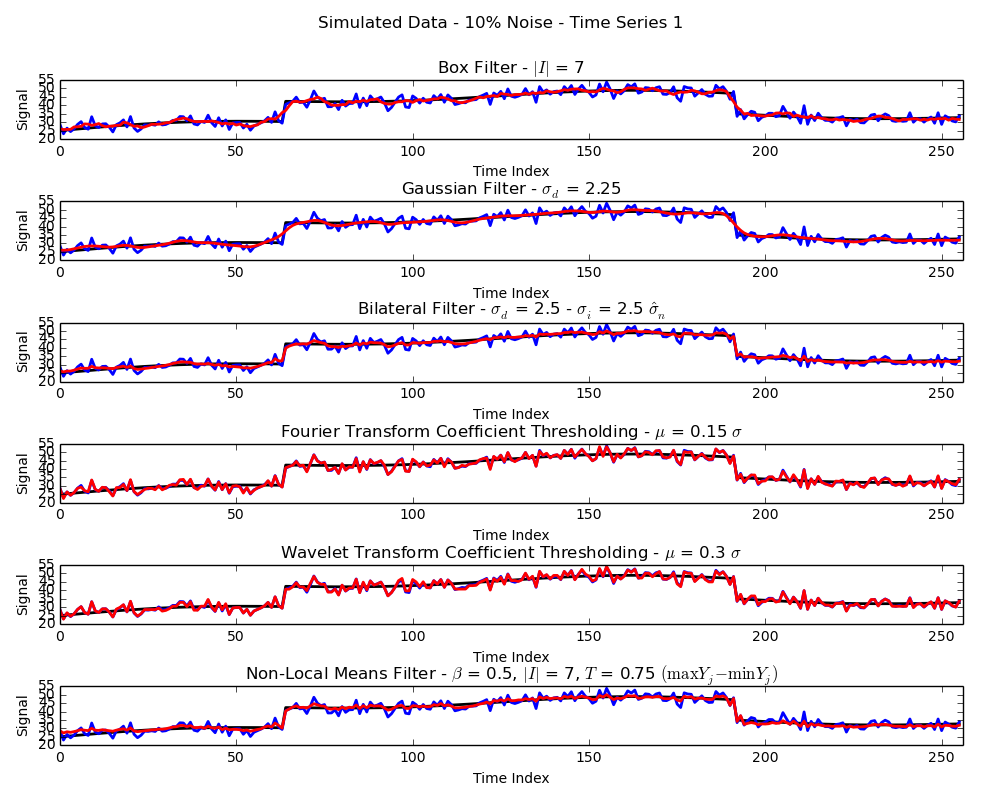
\includegraphics[width = 1 \textwidth,height = 8in]{TimeSeries1SimulatedCompare.png}
\caption{Comparison on Simulated Data - Time Series 1}
\label{timeseries1simulatedcompare}
\end{figure}

\begin{figure}[h!]
\centering
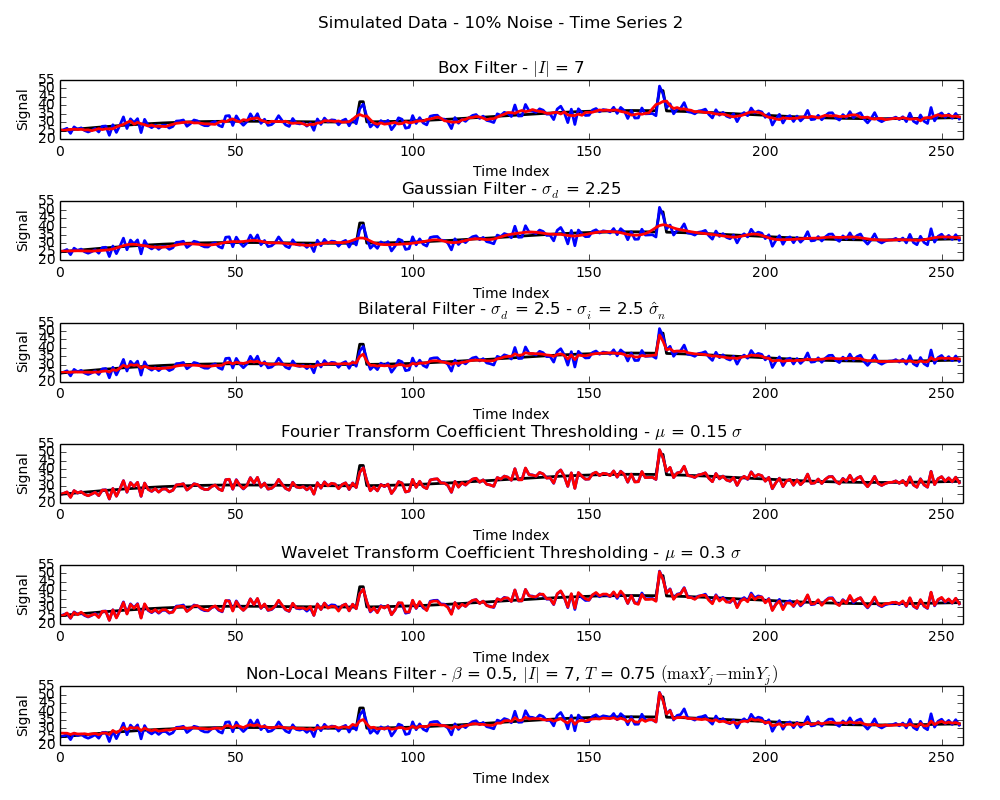
\includegraphics[width = 1 \textwidth,height = 8in]{TimeSeries2SimulatedCompare.png}
\caption{Comparison on Simulated Data - Time Series 2}
\label{timeseries2simulatedcompare}
\end{figure}

\begin{figure}[h!]
\centering
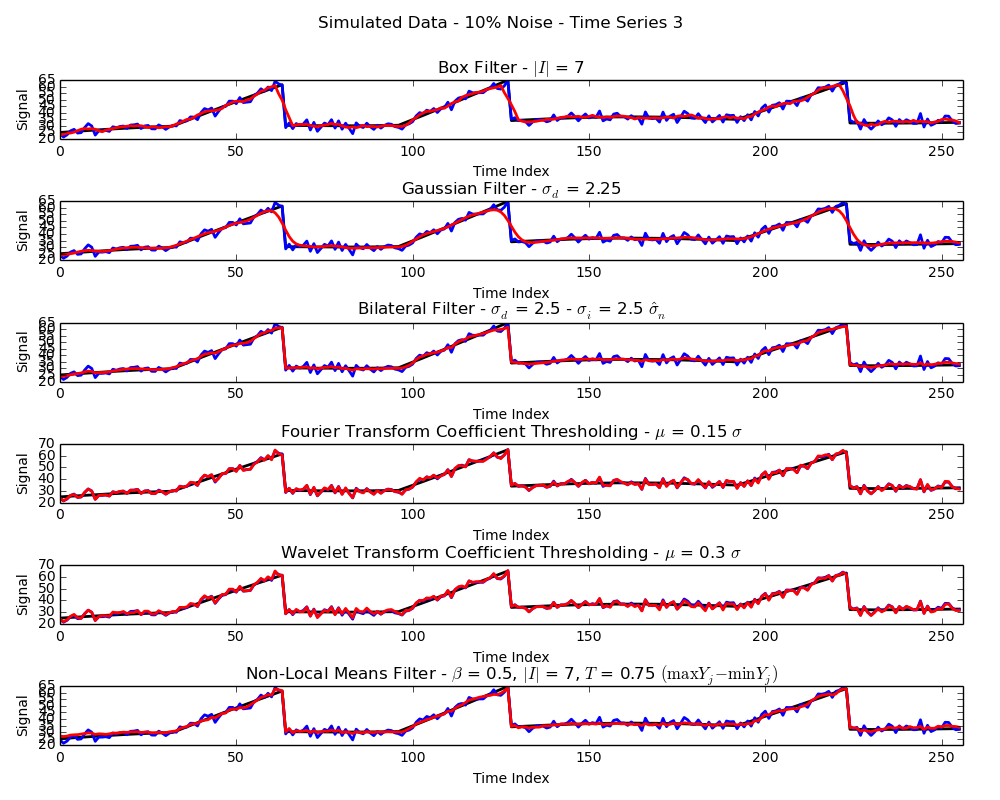
\includegraphics[width = 1 \textwidth,height = 8in]{TimeSeries3SimulatedCompare.png}
\caption{Comparison on Simulated Data - Time Series 3}
\label{timeseries3simulatedcompare}
\end{figure}

%=================================================
\section{Experimental results on real world data}
\label{results2}
%=================================================

Figures \ref{timeseries1realcompare}, \ref{timeseries2realcompare},
and \ref{timeseries3realcompare} show real data that is similar to the
three known time series that were investigated above.

As expected, the box and Gaussian filters destroy features in these
time series while the bilateral filter or non-local means appear to do
well at denoising the time series while retaining features. This can
be seen particularly well at time indices $110$ and $480$ for time
series 1 and at time index $580$ for time series 2.

Fourier transform and wavelet transform coefficient thresholding
appear to do better than expected but denoise less than the
bilateral filter or non-local means for time series 1 and 2.

\begin{figure}[h!]
\centering
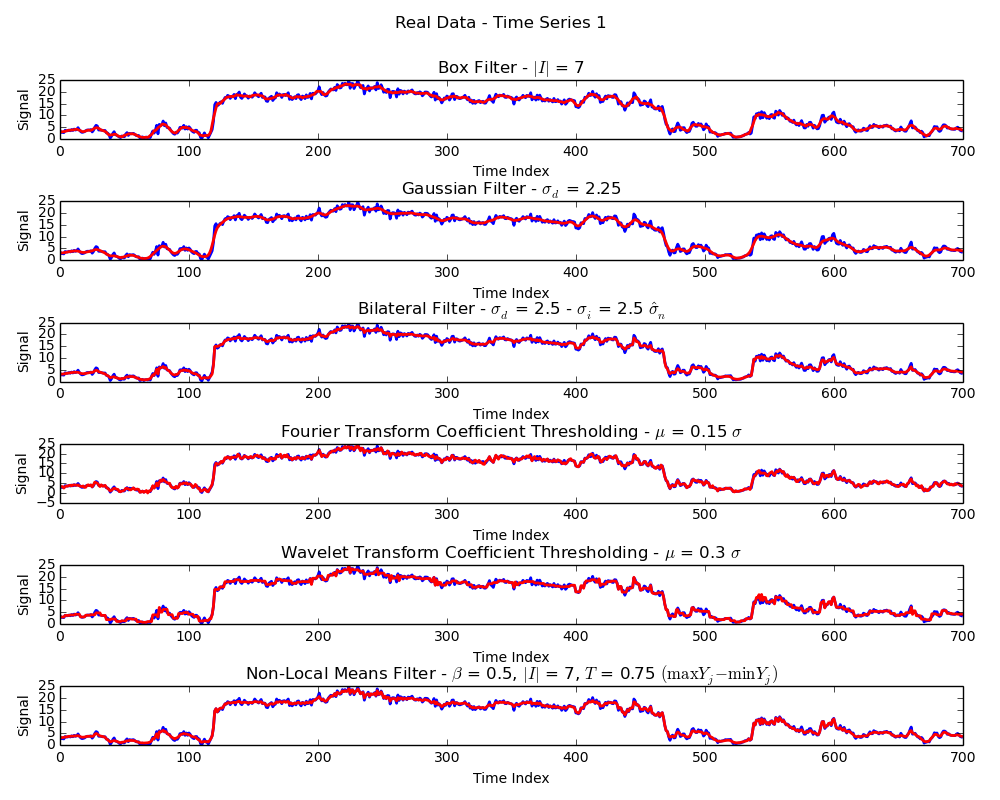
\includegraphics[width = 0.95 \textwidth,height = 8in]{TimeSeries1RealCompare.png}
\caption{Comparison on Real Data - Time Series 1}
\label{timeseries1realcompare}
\end{figure}

\begin{figure}[h!]
\centering
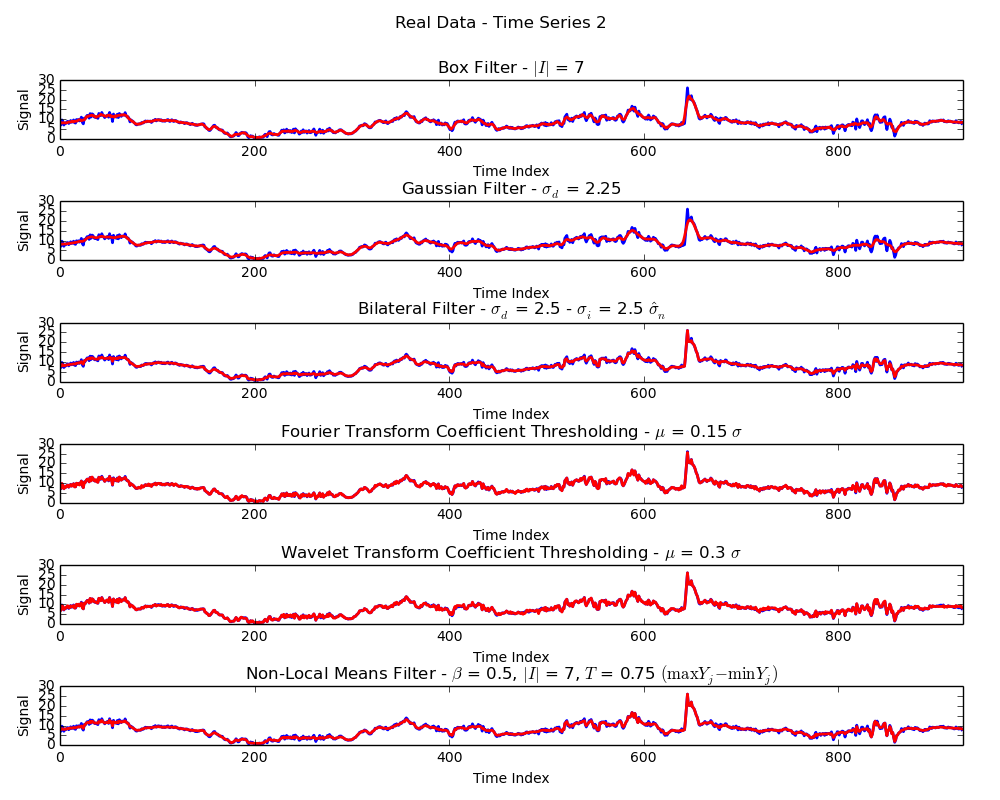
\includegraphics[width = 0.95 \textwidth,height = 8in]{TimeSeries2RealCompare.png}
\caption{Comparison on Real Data - Time Series 2}
\label{timeseries2realcompare}
\end{figure}

\begin{figure}[h!]
\centering
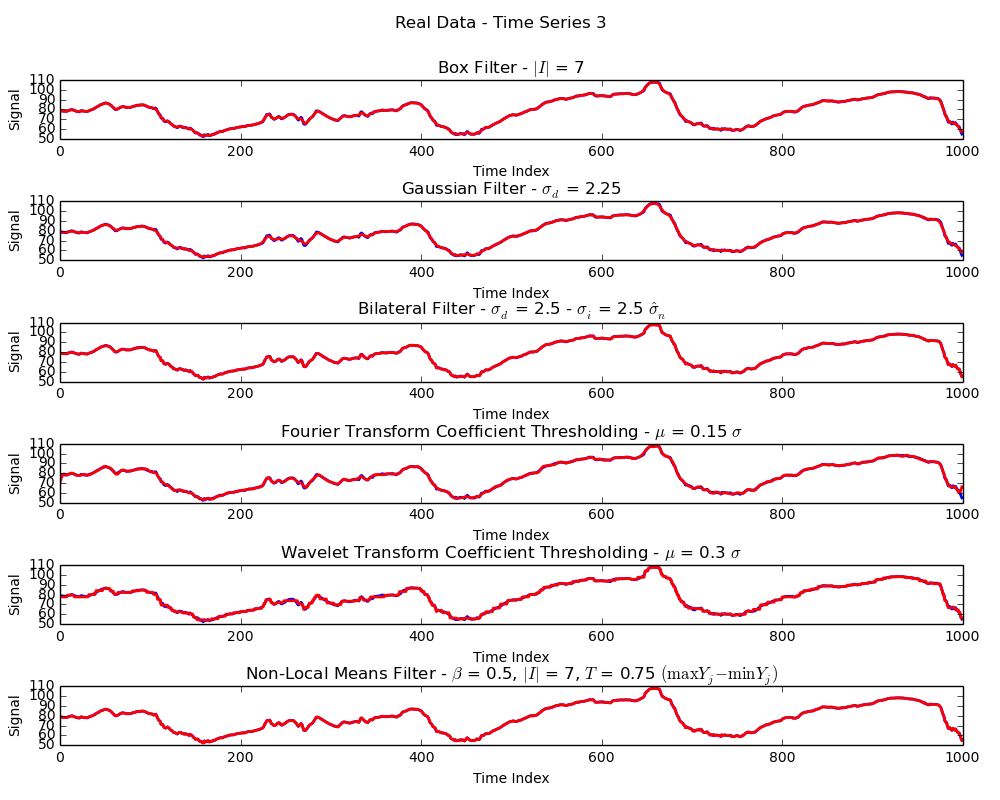
\includegraphics[width = 0.95 \textwidth,height = 8in]{TimeSeries3RealCompare.png}
\caption{Comparison on Real Data - Time Series 3}
\label{timeseries3realcompare}
\end{figure}

%==========================================
\section{Conclusions} \label{conclusion}
%==========================================

The box filter, Gaussian filter, Fourier transform coefficient
thresholding, and wavelet transform coefficient thresholding
consistently offer the worst performance, and all of these methods may
in fact reduce PSNR for the time series. Also, Fourier transform
coefficient thresholding is difficult to implement well for
incremental time series. These techniques are not recommended as
implemented. The wavelet transform can be improved with better choice
of the family of wavelets.

Frequency based techniques such as Fourier transform coefficient
thresholding or wavelet transform coefficient thresholding seem to do
particularly poorly with a fixed parameter value. The more common
practice with frequency techniques is to use SURE or another metric to
fine tune the denoising parameters.

Non-local means offers a consistent improvement in PSNR, but its
performance can be improved by paring it with a bilateral filter. The
parameter $\beta$ has an important impact on the performance of
non-local means. A future area of research should be to determine if
some relationship between the variance of the time series and the
estimated noise variance could be used to chose $\beta$. Also,
non-local means should theoretically perform better with longer time
series, where more matching neighborhoods are possible. This
possibility should be investigated. It is important to keep in mind
that there is a tradeoff between keeping the data set small to ensure
reasonable computation time and providing sufficient data to ensure
good performance for non-local means.

One or two iterations of the same bilateral filter appears to offer
the best consistent performance. Both have relatively stable optimal
parameter settings, with a single iteration of the bilateral filter
being slightly more stable. Other versions of multiple iterations of a
bilateral filter offer less consistent results.

Note that only Gaussian white noise was considered in this paper. In future work, non-Gaussian noise will be considered in the experiments for parameter settings. Instead of the design of experiments used in this paper, possible methods that could automatically find thresholds or parameters for denoising methods will also be explored.

% Future work?

\section*{Acknowledgment}
This work performed under the auspices of the U.S.  Department of
Energy by Lawrence Livermore National Laboratory (LLNL) under Contract
DE-AC52-07NA27344.  This work was part of the SensorStreams project at
LLNL. Jeremy Luke Thompson was a visiting faculty member from the U.S. Air Force Academy when working on this project at LLNL during the summer of 2014.

\FloatBarrier

%\bibliographystyle{acm}
\bibliographystyle{plain}
\bibliography{notes}

\end{document}
